\documentclass[aspectratio=1610, 10pt, notheorems]{beamer}
\usetheme{Warsaw} 
\usecolortheme{seahorse}

%%% Кодировка и локализация %%%
\usepackage[utf8]{inputenc} % кодовая страница документа
\usepackage[T2A]{fontenc} % внутренняя кодировка  TeX
\usepackage[english,russian]{babel} % локализация и переносы

%%% Гипперссылки и pdf %%%
\usepackage{cmap} % русский поиск в pdf
\usepackage{hyperref} % гиперссылки

%%% Пакеты для формул %%%
\usepackage{amsmath} % удобная вёрстка многострочных формул, масштабирующийся текст в формулах, формулы в рамках и др.
\usepackage{amssymb} % несколько сотен дополнительных математических символов
\usepackage{amsthm} % окружения «теорема», «лемма» и т. п.
\usepackage{amsfonts} % Ажурный \mathbb{} и готический \mathfrak{} шрифты
\usepackage{mathrsfs} % Mathematical Script letters (шрифт Эйлера) \mathscr{}
\usepackage{euscript} % Шрифт Евклида \EuScript{}
% каллиграфический шрифт \mathcal{} не требует пакета
\usepackage{enumitem}
\usepackage{bm}
\usepackage{multicol}

%%% Графика, изображения и цвета %%%
\usepackage{graphicx} % Работа с графикой \includegraphics{}
\usepackage{float} % Фиксация плавабщих боксов [H]
\graphicspath{
    {./images/}, 
    {./images/img1/}, 
    {./images/img2/}, 
    {./images/img3/}, 
    {./images/tikz1/}, 
    {./images/tikz2/}, 
    {./images/tikz3/},
    {./images/tree/},
    {./images/presentation/},
    }
    
\newtheorem{theorem}     {Теорема}
\newtheorem{lemma}       {Лемма}
\newtheorem{proposition} {Предложение}
\newtheorem{corollary}   {Следствие}
\newtheorem{definition}  {Определение}
\newtheorem{example}     {Пример} 
\newtheorem{remark}      {Замечание}
   
%%% Настройки презентации %%%
\everymath{\color{blue}}    % цвет формул в текстмоде
\everydisplay{\color{blue}} % цвет выключных формул
\setbeamertemplate{navigation symbols}{} % Убрать панель навигации
% \setbeamertemplate{footline}[frame number] % Номера слайдов вместо нижней строки
\setbeamertemplate{page number in head/foot}[totalframenumber]
\setbeamertemplate{bibliography item}{\insertbiblabel}
\hypersetup{unicode=true} % разрешить использование символов Юникод в закладках. настройка для hiperref

%%% Русская традиция начертания математических знаков
\renewcommand{\le}  {\ensuremath{\leqslant}}
\renewcommand{\leq} {\ensuremath{\leqslant}}
\renewcommand{\ge}  {\ensuremath{\geqslant}}
\renewcommand{\geq} {\ensuremath{\geqslant}}
\renewcommand{\emptyset}{\varnothing}

%%% Русская традиция начертания математических функций (на случай копирования из зарубежных источников)
\renewcommand{\tan}{\operatorname{tg}}
\renewcommand{\cot}{\operatorname{ctg}}
\renewcommand{\csc}{\operatorname{cosec}}

%%% Русская традиция начертания греческих букв (греческие буквы вертикальные, через пакет upgreek)
% \usepackage{upgreek} % прямые греческие ради русской традиции
% \renewcommand{\epsilon}{\ensuremath{\upvarepsilon}}   %  русская традиция записи
% \renewcommand{\phi}{\ensuremath{\upvarphi}}
% %\renewcommand{\kappa}{\ensuremath{\varkappa}}
% \renewcommand{\alpha}{\upalpha}
% \renewcommand{\beta}{\upbeta}
% \renewcommand{\gamma}{\upgamma}
% \renewcommand{\delta}{\updelta}
% \renewcommand{\varepsilon}{\upvarepsilon}
% \renewcommand{\zeta}{\upzeta}
% \renewcommand{\eta}{\upeta}
% \renewcommand{\theta}{\uptheta}
% \renewcommand{\vartheta}{\upvartheta}
% \renewcommand{\iota}{\upiota}
% \renewcommand{\kappa}{\upkappa}
% \renewcommand{\lambda}{\uplambda}
% \renewcommand{\mu}{\upmu}
% \renewcommand{\nu}{\upnu}
% \renewcommand{\xi}{\upxi}
% \renewcommand{\pi}{\uppi}
% \renewcommand{\varpi}{\upvarpi}
% \renewcommand{\rho}{\uprho}
% %\renewcommand{\varrho}{\upvarrho}
% \renewcommand{\sigma}{\upsigma}
% %\renewcommand{\varsigma}{\upvarsigma}
% \renewcommand{\tau}{\uptau}
% \renewcommand{\upsilon}{\upupsilon}
% \renewcommand{\varphi}{\upvarphi}
% \renewcommand{\chi}{\upchi}
% \renewcommand{\psi}{\uppsi}
% \renewcommand{\omega}{\upomega}



\newcommand {\rr}  {\mathbb{R}}
\newcommand {\nn}  {\mathbb{N}}
\newcommand {\zz}  {\mathbb{Z}}
\newcommand {\bbc} {\mathbb{C}}
% \newcommand {\rd}  {\mathbb{R}^d}
% \newcommand {\rpo} {\mathbb{R}_+^1}

\newcommand {\al} {\alpha}
\newcommand {\be} {\beta}
\newcommand {\da} {\delta}
\newcommand {\Da} {\Delta}
\newcommand {\Dl} {\Delta}
\newcommand {\ga} {\gamma}
\newcommand {\Ga} {\Gamma}
\newcommand {\la} {\lambda}
\newcommand {\La} {\Lambda}
\newcommand {\om} {\omega}
\newcommand {\Om} {\Omega}
\newcommand {\sa} {\sigma}
\newcommand {\Sa} {\Sigma}
\newcommand {\te} {\theta}
\newcommand {\fy} {\varphi}
\newcommand {\Fy} {\varPhi}
\newcommand {\ep} {\varepsilon}
\newcommand {\ro} {\varrho}

\newcommand{\bd}{{\bm{d}}}
\newcommand{\bj}{{\bm{j}}}
\newcommand{\bi}{{\bm{i}}}
\newcommand{\bk}{{\bm{k}}}
\newcommand{\bu}{{\bm{u}}}
\newcommand{\bx}{{\bm{x}}}
\newcommand{\bl}{{\bf{l}}}
\newcommand{\bma}{{\bm{\alpha}}}
\newcommand{\bmb}{{\bm{\beta}}}
\newcommand{\bmg}{{\bm{\gamma}}}

\newcommand {\ra}  {\rightarrow}
\newcommand {\IN}  {\subset}
\newcommand {\NI}  {\supset}
\newcommand {\mmm} {\setminus}
\newcommand {\8}   {\infty}
\newcommand {\io}  {I^\infty}
\newcommand {\ia}  {I^*}
\newcommand {\0}   {\varnothing}
\newcommand {\dd}  {\partial}
\newcommand {\pr}  {\mathrm{pr}}
% \renewcommand{\span}{\mathrm{span}}


\newcommand {\eA} {{\EuScript A}}
\newcommand {\eJ} {{\EuScript J}}
\newcommand {\eC} {{\EuScript C}}
\newcommand {\eU} {{\EuScript U}}
\newcommand {\eP} {{\EuScript P}}
\newcommand {\eS} {{\EuScript S}}
\newcommand {\eW} {{\EuScript W}}
\newcommand {\eZ} {{\EuScript Z}}
\newcommand {\eK} {{\EuScript K}}
\newcommand {\hT} {{\hat T}}
\newcommand {\wP} {{\widetilde P}}
\newcommand {\eV} {{\mathcal V}}

\def \diam {\mathop{\rm diam} \nolimits}
\def \sup  {\mathop{\rm sup}  \nolimits}
\def \fix  {\mathop{\rm fix}  \nolimits}
\def \Lip  {\mathop{\rm Lip}  \nolimits}
\def \min  {\mathop{\rm min}  \nolimits}
\def \Ln   {\mathop{\rm Ln}   \nolimits}
\def \Id   {\mathop{\rm Id}   \nolimits}

\newcommand{\red}{\textcolor{red}}     % Новые переменные и переименования

%%% Данные для титульного листа %%%
\title[Анализ на самоподобных множествах с конечным пересечением]
    {Анализ на самоподобных множествах с конечным пересечением}
\author[Дмитрий Дроздов]
    {Дроздов Дмитрий Алексеевич\\ \; \\
    Научный руководитель:\\ 
    д-р физ.-мат. наук, доц.
    Тетенов Андрей Викторович}
\institute[ИМ СО РАН]{Институт математики имени С. Л. Соболева СО РАН}
\date[10.06.2024]
    {Семинар <<Геометрия, топология и их приложения>>\\ \; \\
    10.06.2024}


\begin{document}


\begin{frame}{}
    \titlepage
\end{frame}

\begin{frame}{}
\Huge{Часть 1.\\
Деформации полигональных систем}
\end{frame}

\begin{frame}{Актуальность}
\begin{thebibliography}{9}

\bibitem{Hut1981}{
    {\sc J. Hutchinson,}
    {\it Fractals and {S}elf-{S}imilarity,}
    {Indiana University Mathematics Journal (5) \textbf{30} (1981) 713--747}}
    
\bibitem{Hata1985}{
    {\sc M. Hata,}
    {\it On the structure of self-similar sets,}
    {Japan Journal of Applied Mathematics (2) \textbf{2} (1985) 381--414}}

\bibitem{SSS2}{
    {\sc C. Bandt, K. Keller,}
    {\it Self‐Similar Sets 2. A Simple Approach to the Topological Structure of Fractals,}
    {Mathematische Nachrichten (1) \textbf{154} (1991) 27--39}}

\bibitem{Strichartz1999}{
    {\sc R. Strichartz,}
    {\it Isoperimetric Estimates on Sierpinski Gasket Type Fractals}
    {Transactions of the American Mathematical Society (5) \textbf{135} (1999) 1705--1752}}

\bibitem{strich1999}{
    {\sc R. Strichartz,}
    {\it Analysis on fractals}
    {Notices AMS (10) \textbf{46} (1999) 1199--1208}}

\bibitem{6}{
    {\sc А. В. Тетенов, М. С. Самуэль, Д. А. Ваулин,}
    {\it О дендритах, заданных системами полиэдров и их точках ветвления,}
    {Труды Института математики и механики УрО РАН (4) \textbf{23} (2017) 281--291}}

\bibitem{7}{
    {\sc M. Samuel, A. V. Tetenov, D. A. Vaulin,}
    {\it Self-similar dendrites generated by polygonal systems in the plane,}
    {Siberian Electronic Mathematical Reports \textbf{14} (2017) 737--751}}

\bibitem{8}{
    {\sc A. Tetenov,}
    {\it Finiteness properties for self-similar continua,}
    {arXiv:2003.04202 (2021)}}

\end{thebibliography}
\end{frame}


\begin{frame}{Цели и выносимые на защиту положения}
Цель:
\begin{enumerate}
\item[$\bullet$] Обобщить класс полигональных дендритов.
\end{enumerate}

\hfill

Выносимые на защиту положения:
\begin{enumerate}
\item[1] Для обобщённой полигональной системы, являющейся $\delta$-деформацией стягиваемой полигональной системы, найдено необходимое условие того, что её аттрактор будет дендритом (с одноточечным пересечением);
\item[2] Доказано существование такого $\delta$, что для аттрактор любой $\delta$-деформации, удовлетворяющей условию совпадения параметров, является дендритом.
\end{enumerate}
\end{frame}


\begin{frame}{Самоподобное множество}

\only<1>{
    \begin{definition}[Hutchinson J. E. (1981)]
        Пусть $\eS=\{S_1, \ldots, S_m\}$ --- система сжимающих подобий в $\mathbb{R}^n$.  
        Непустой компакт $K$, удовлетворяющий уравнению  $K=\bigcup\limits_{i=1}^m S_i(K)$, будем называть {\em аттрактором системы} $\eS$ или множеством, самоподобным (инвариантным) относительно системы $\eS$.
    \end{definition}
    \begin{block}{}
        Для системы $\eS=\{S_1,\ldots,S_r\}$ сжимающих подобий в $\rr^k$  равенством $T(A)=\bigcup\limits_{i=1}^r S_i(A)$ задётся соответствующий оператор Хатчинсона на $C(\rr^k)$.
    \end{block}
    Мы обозначим как $I=\{1, \ldots, m\}$ множество индексов системы $\eS$, а также обозначим как $I^{*}=\bigcup\limits_{n=1}^\infty I^n$ множество слов $\bm{i}=i_1\ldots i_n$ конечной длинны алфавита $I$, называемых {\em мультииндексами}.
    Мы будем использовать сокращение $S_{\bj} = S_{j_{1}j_{2}\ldots j_{n}}=S_{j_{1}}S_{j_{2}} \ldots S_{j_{n}}$ и обозначим $S_{\bj}(K)$ как $K_{\bj}$.
    Множество $K_\bj$,  где $\bj=j_{1}j_{2}\ldots j_{n}$,  будем называть {\em копией порядка (итерации) $n$} множества $K$.
    \footnotetext[1]{Hutchinson J. E., Fractals and self-similarity, Indiana Univ. Math. J. \textbf{30} (1981), 713--747.}}
\only<2>{
    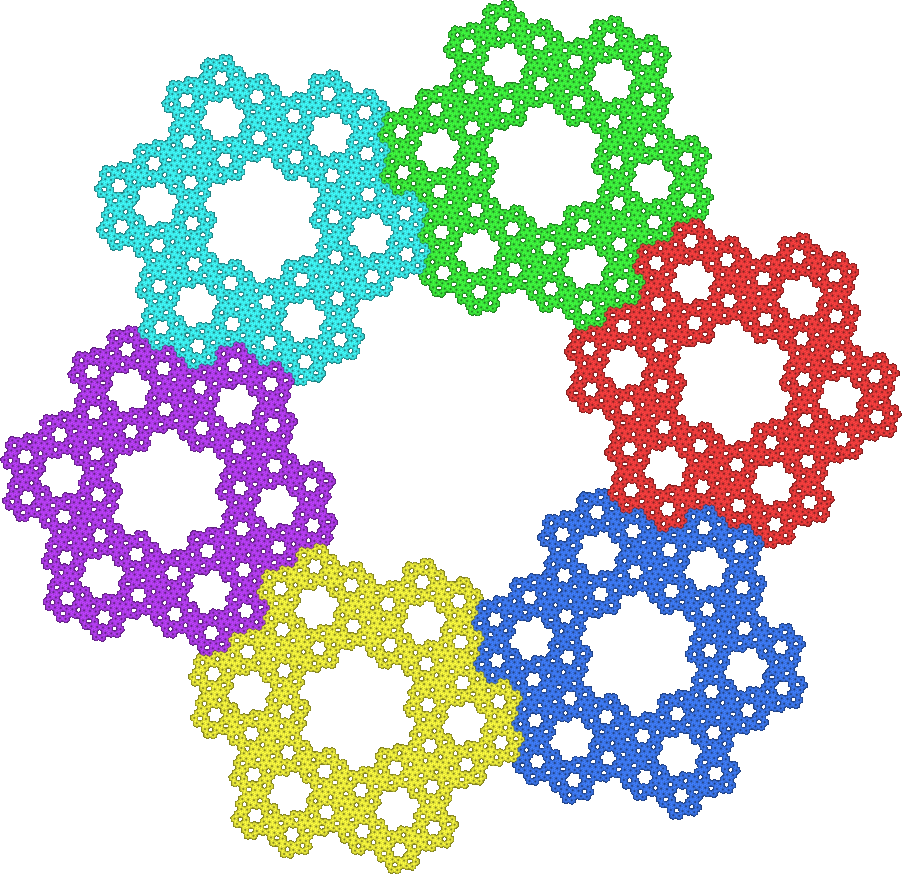
\includegraphics[width=0.4\textwidth]{GosperCarpet.png}
    \hfill
    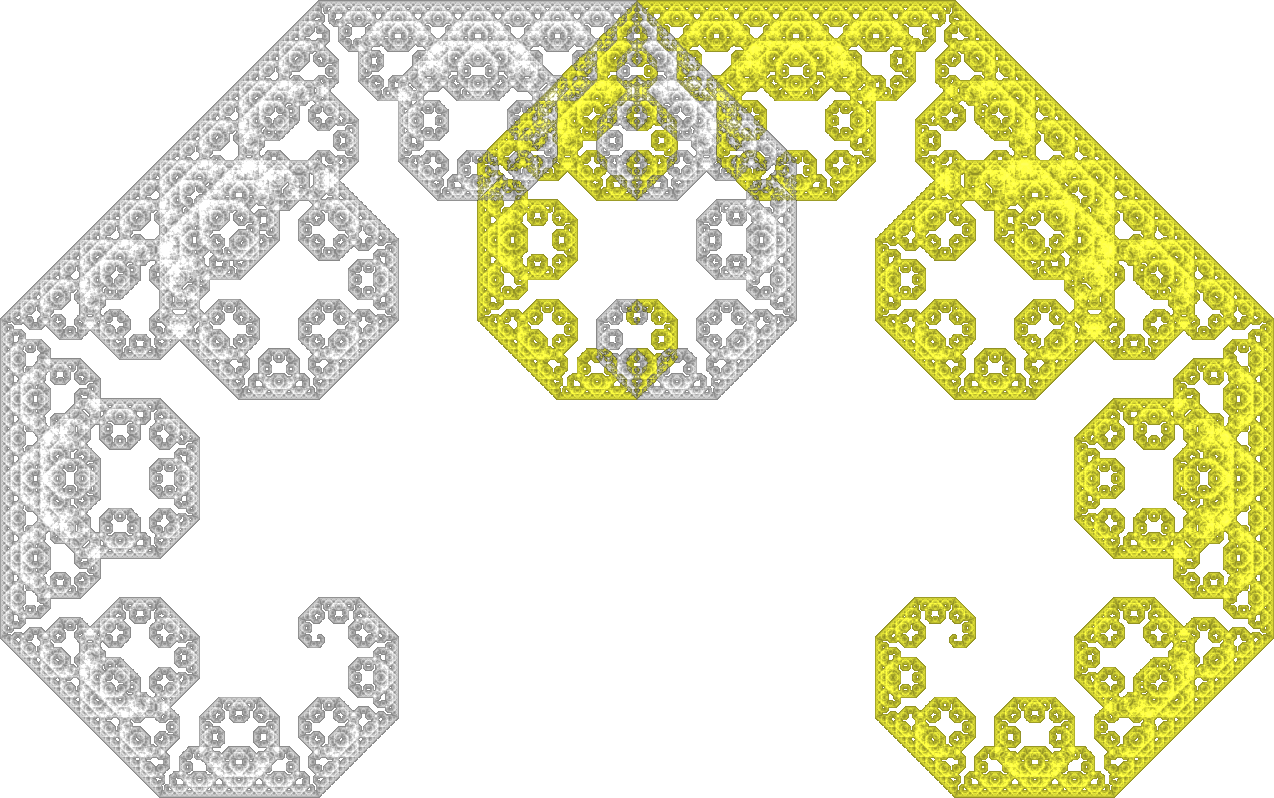
\includegraphics[width=0.55\textwidth]{LevyCurve.png}}
\end{frame}





\begin{frame}{Дендрит}
\begin{definition} 
Дендритом называется локально связный континуум, не содержащий простых замкнутых дуг.
\end{definition}

Пусть $X$ --- дендрит. Тогда из определения дендрита следует, что $X$ односвязно, и что для любых двух точек $x,y \in X$ существует единственная кривая $\gamma$, соединяющая $x$ и $y$.
\end{frame}


\begin{frame}{Стягиваемые $P$-полигональные  системы}
Даны многоугольник $P\IN \mathbb R^2$, множество его вершин $V_P=\{A_1,...,A_{n_P}\}$  и такая система подобий $\eS = \{S_1, \ldots, S_m\}$ в $\mathbb R^2$, что:\\
\only<1>{\[ 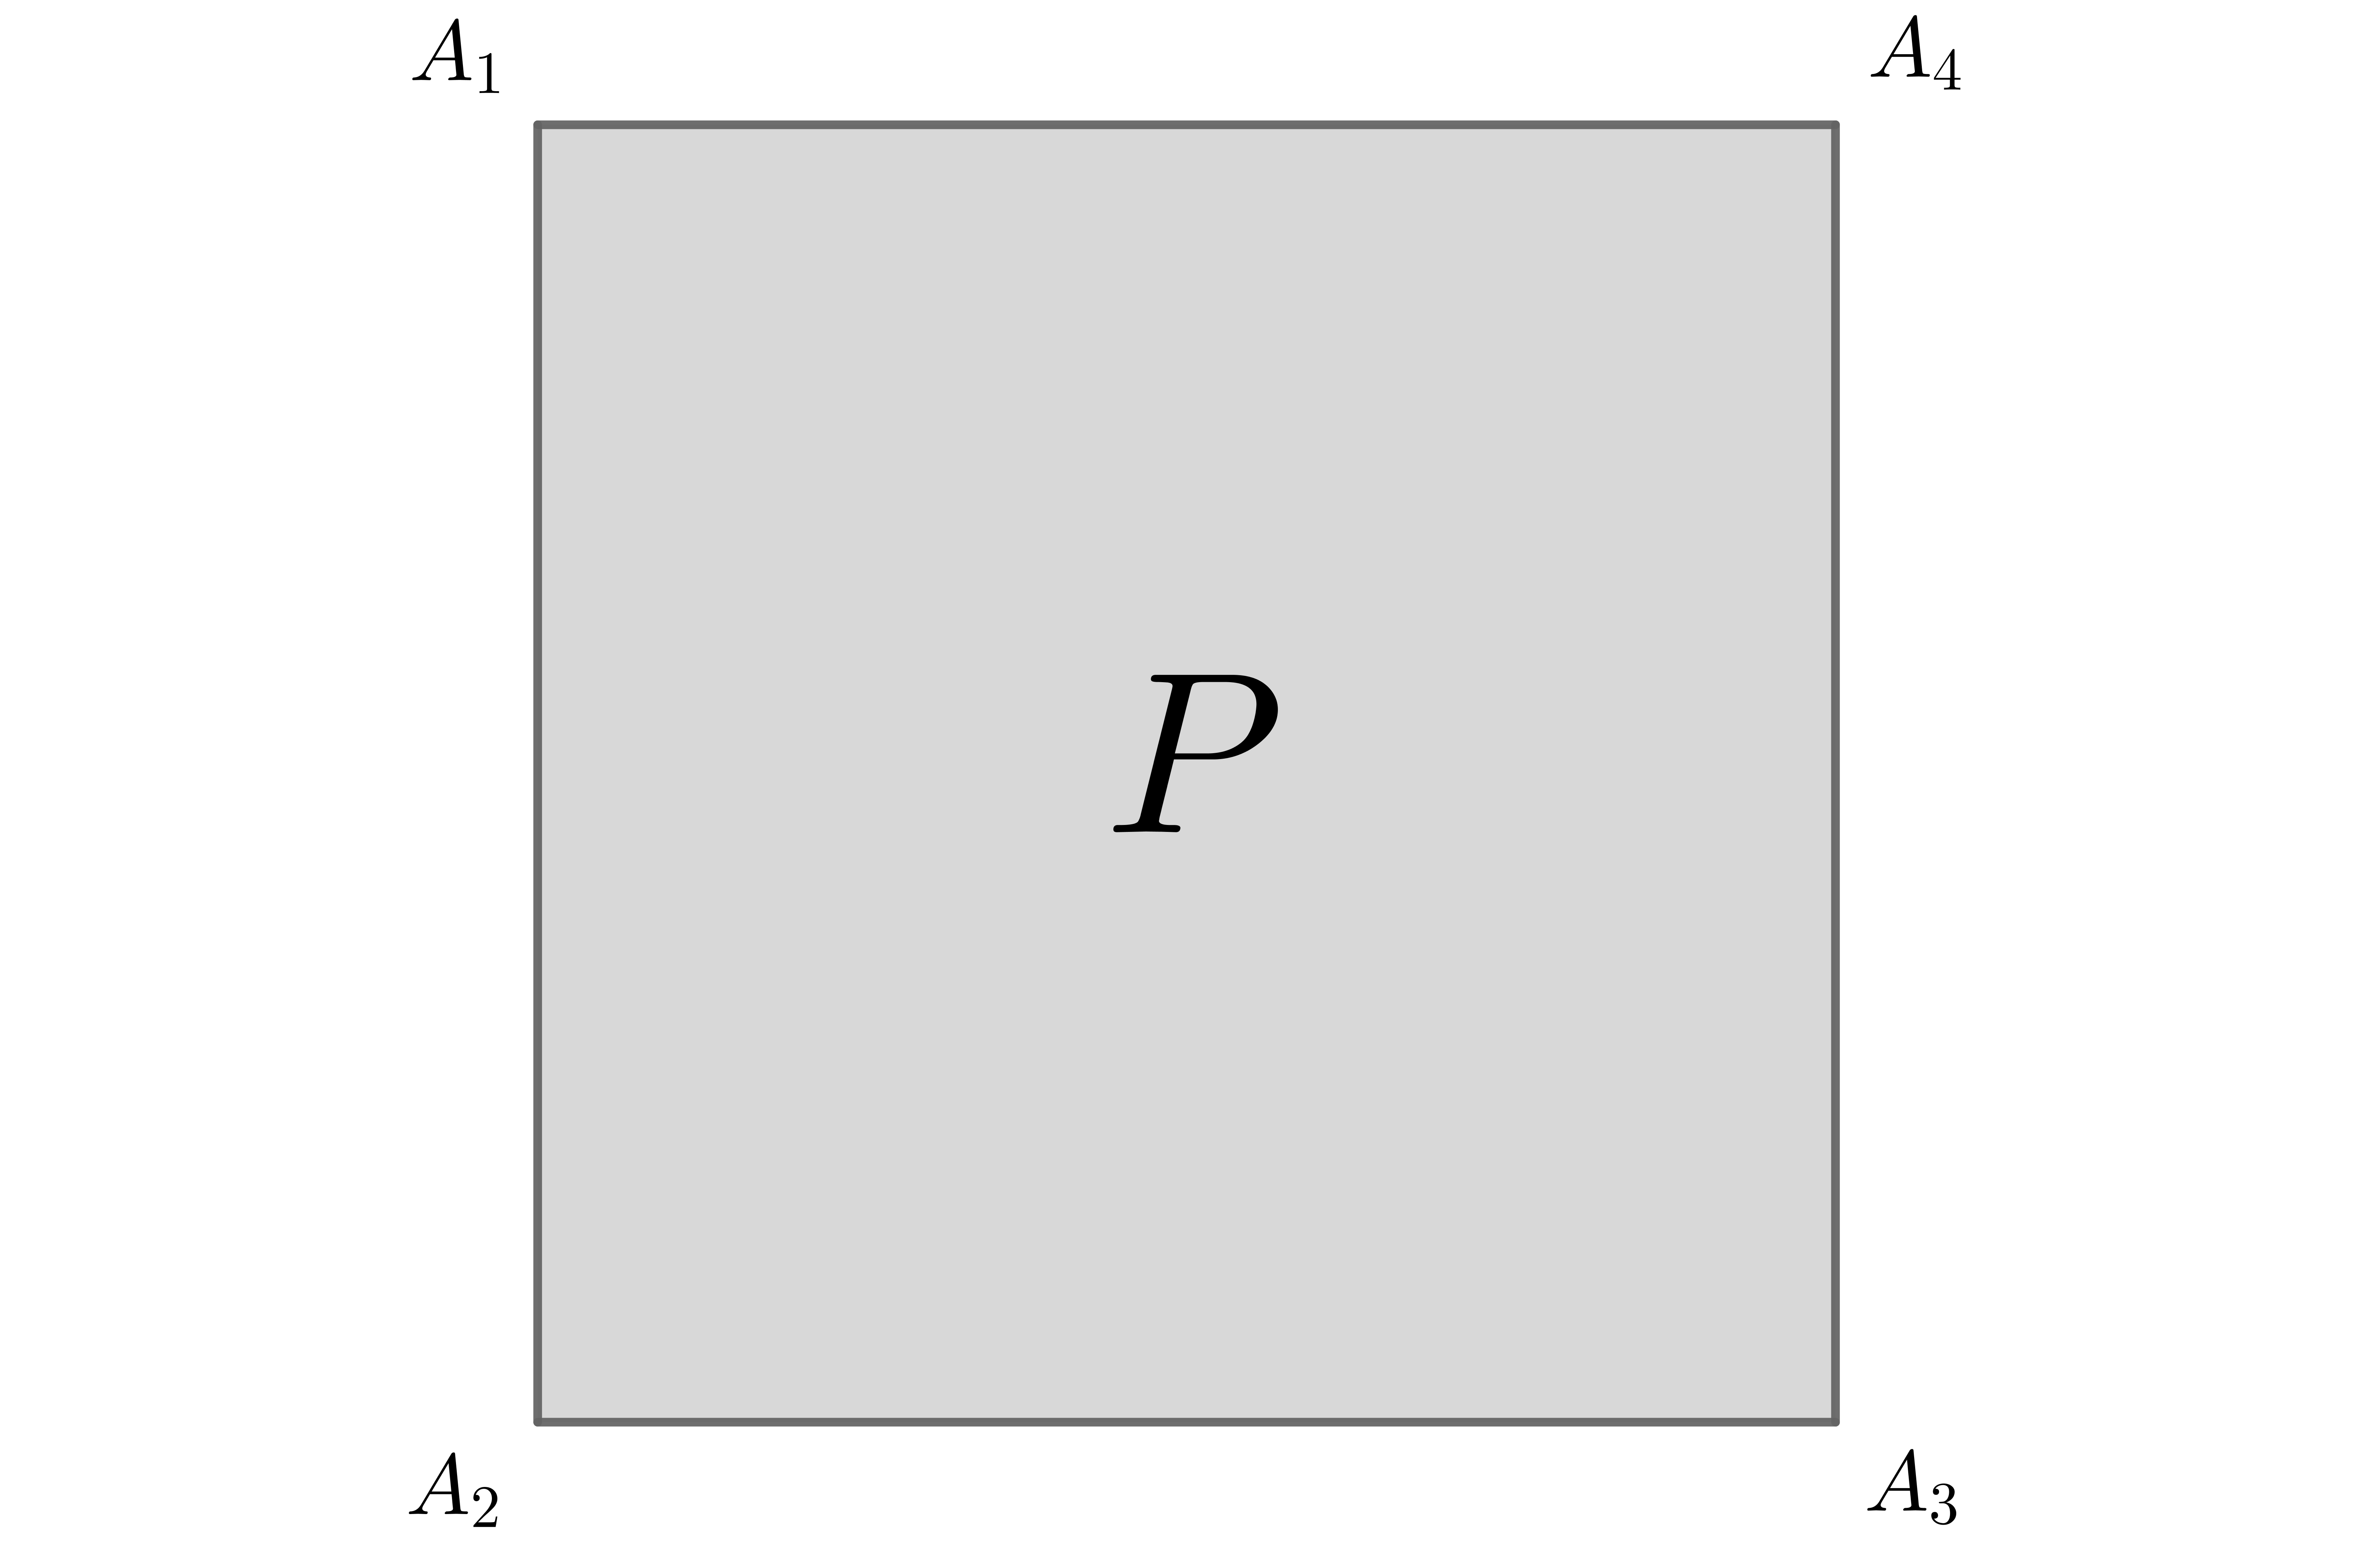
\includegraphics[width=.7\textwidth]{presentation/2_11.png}\]}
\only<2>{
    {\bf(D1)}  для любого $i\in I$, множество $P_i=S_i(P)\IN P$;\\
\[ 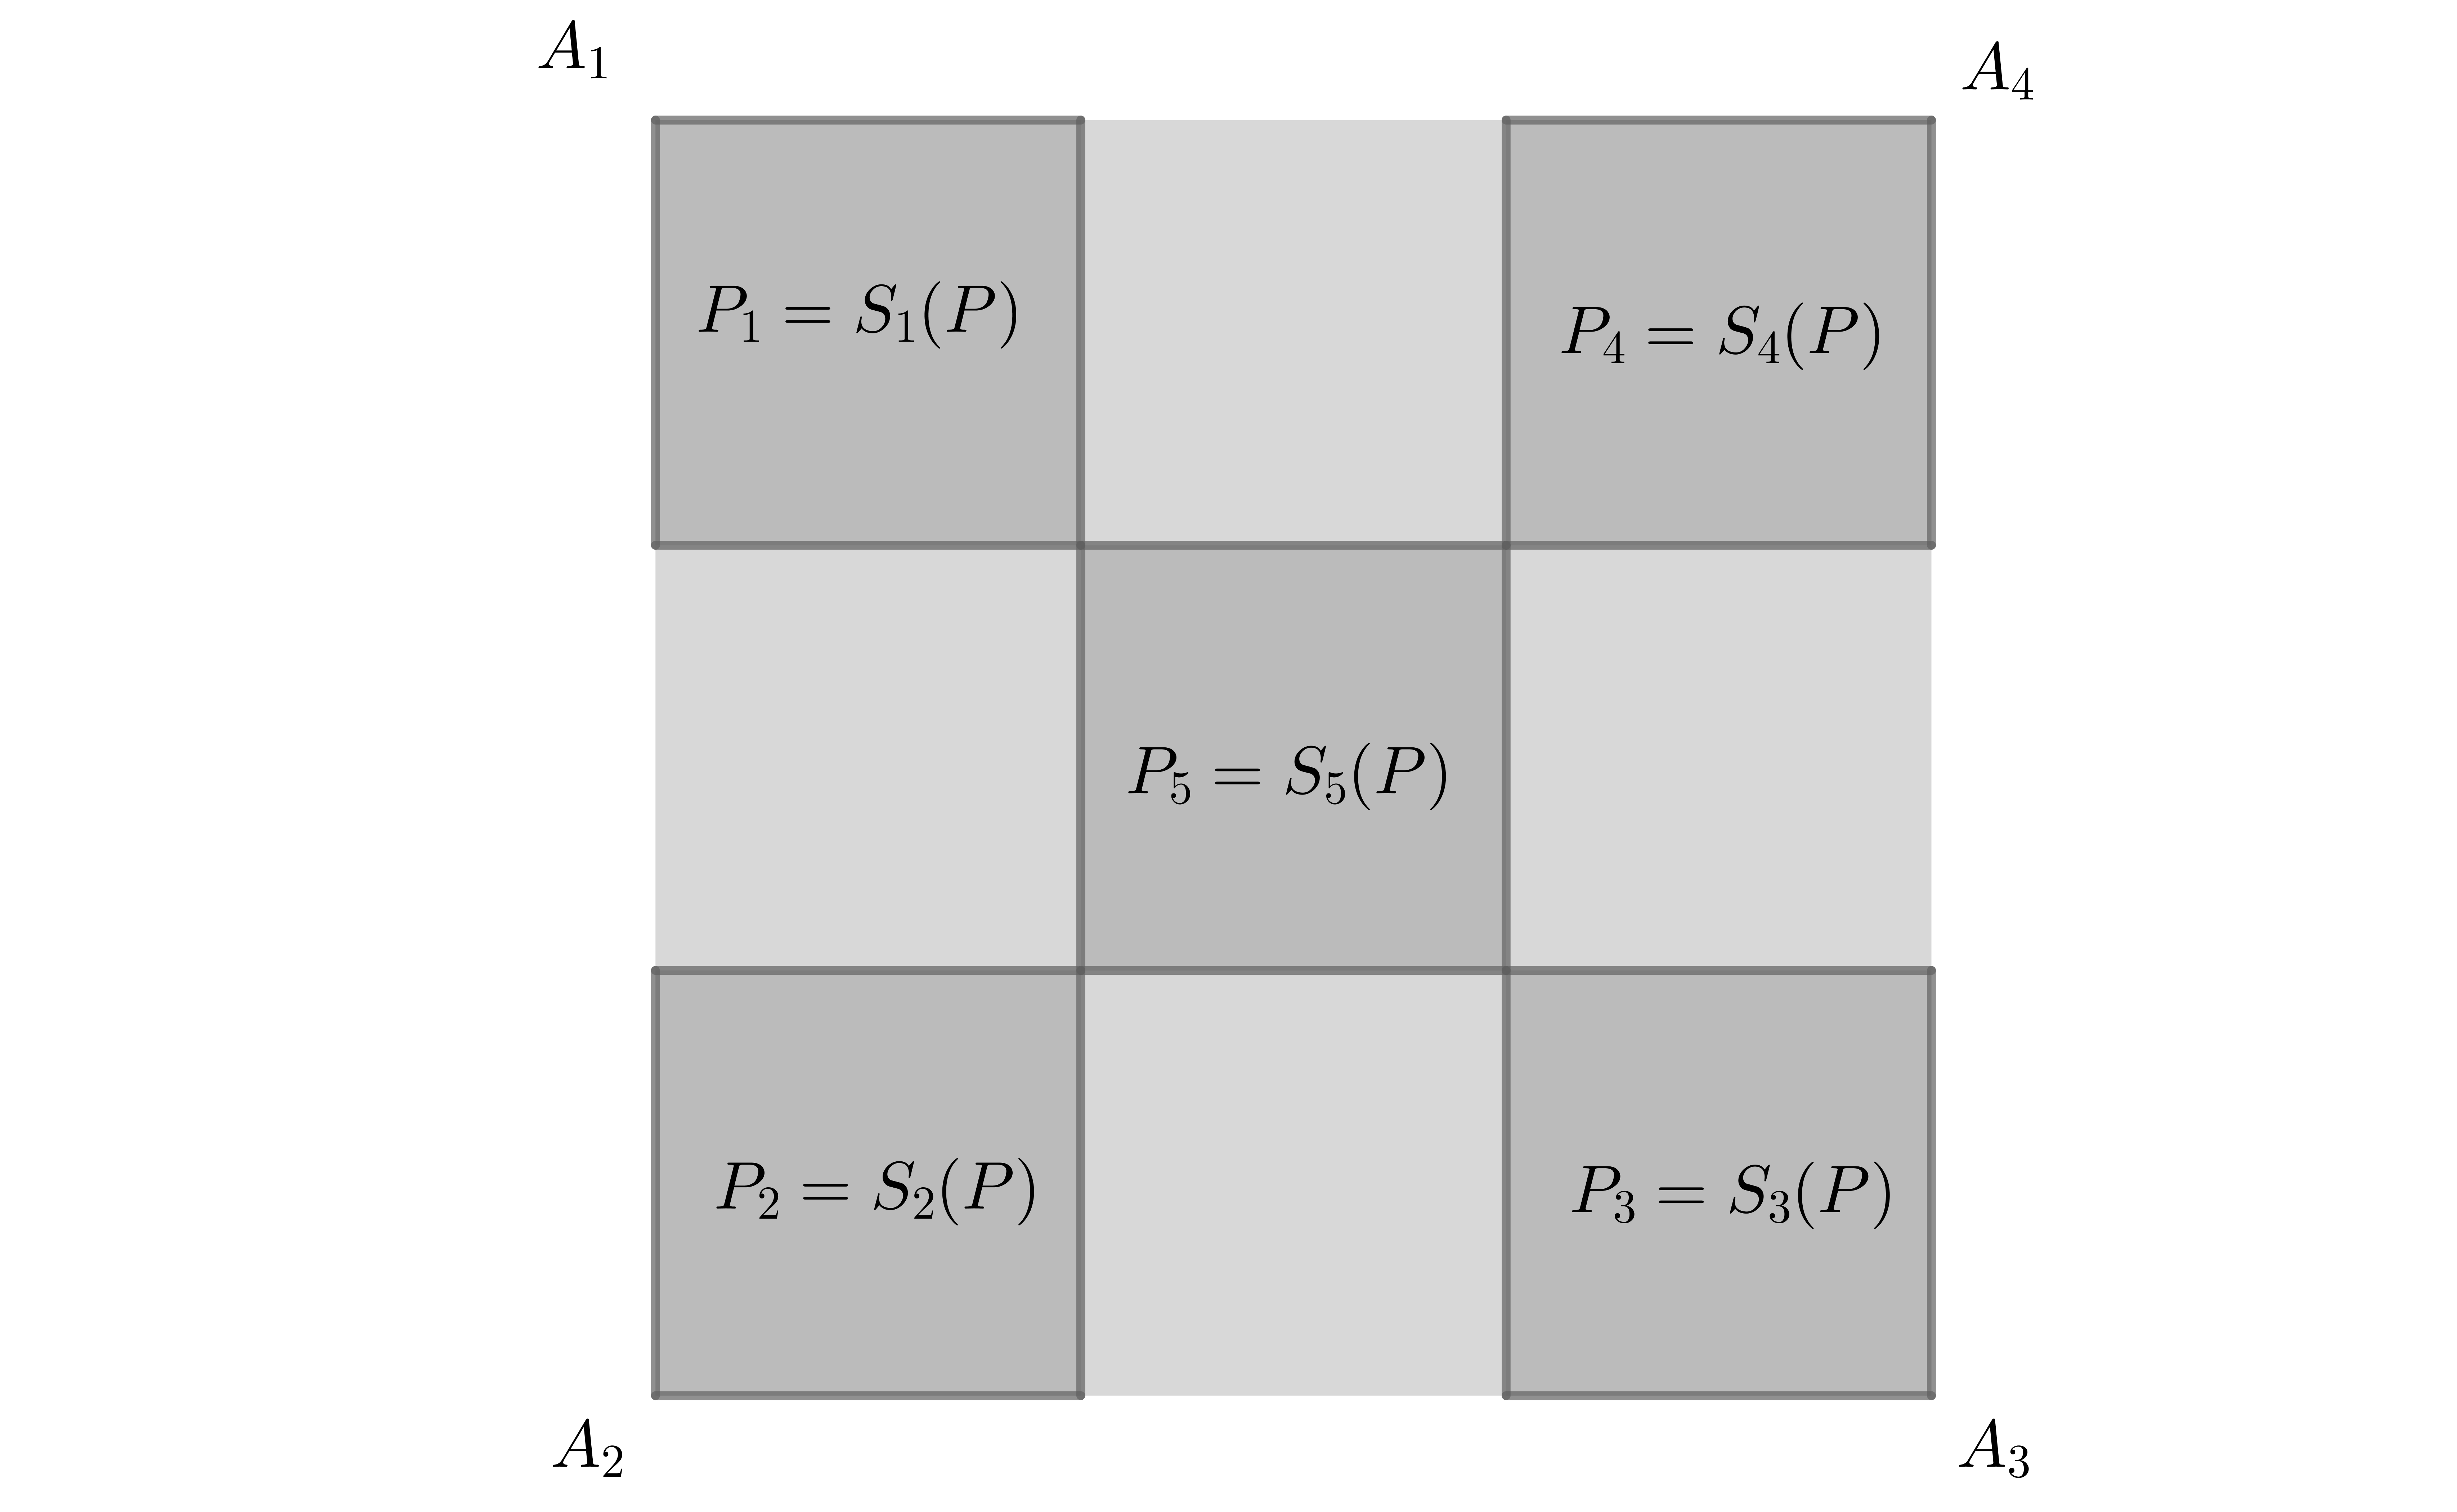
\includegraphics[width=.7\textwidth]{2_22.png}\]}
\only<3>{
{\bf(D1)}  для любого $i\in I$, множество $P_i=S_i(P)\IN P$;\\
{\bf(D2)}  для любых $i\neq j,\ \   i, j \in I,$ $P_i \cap P_j=V_{P_i}\cap V_{P_j}$ ;\\
\[ 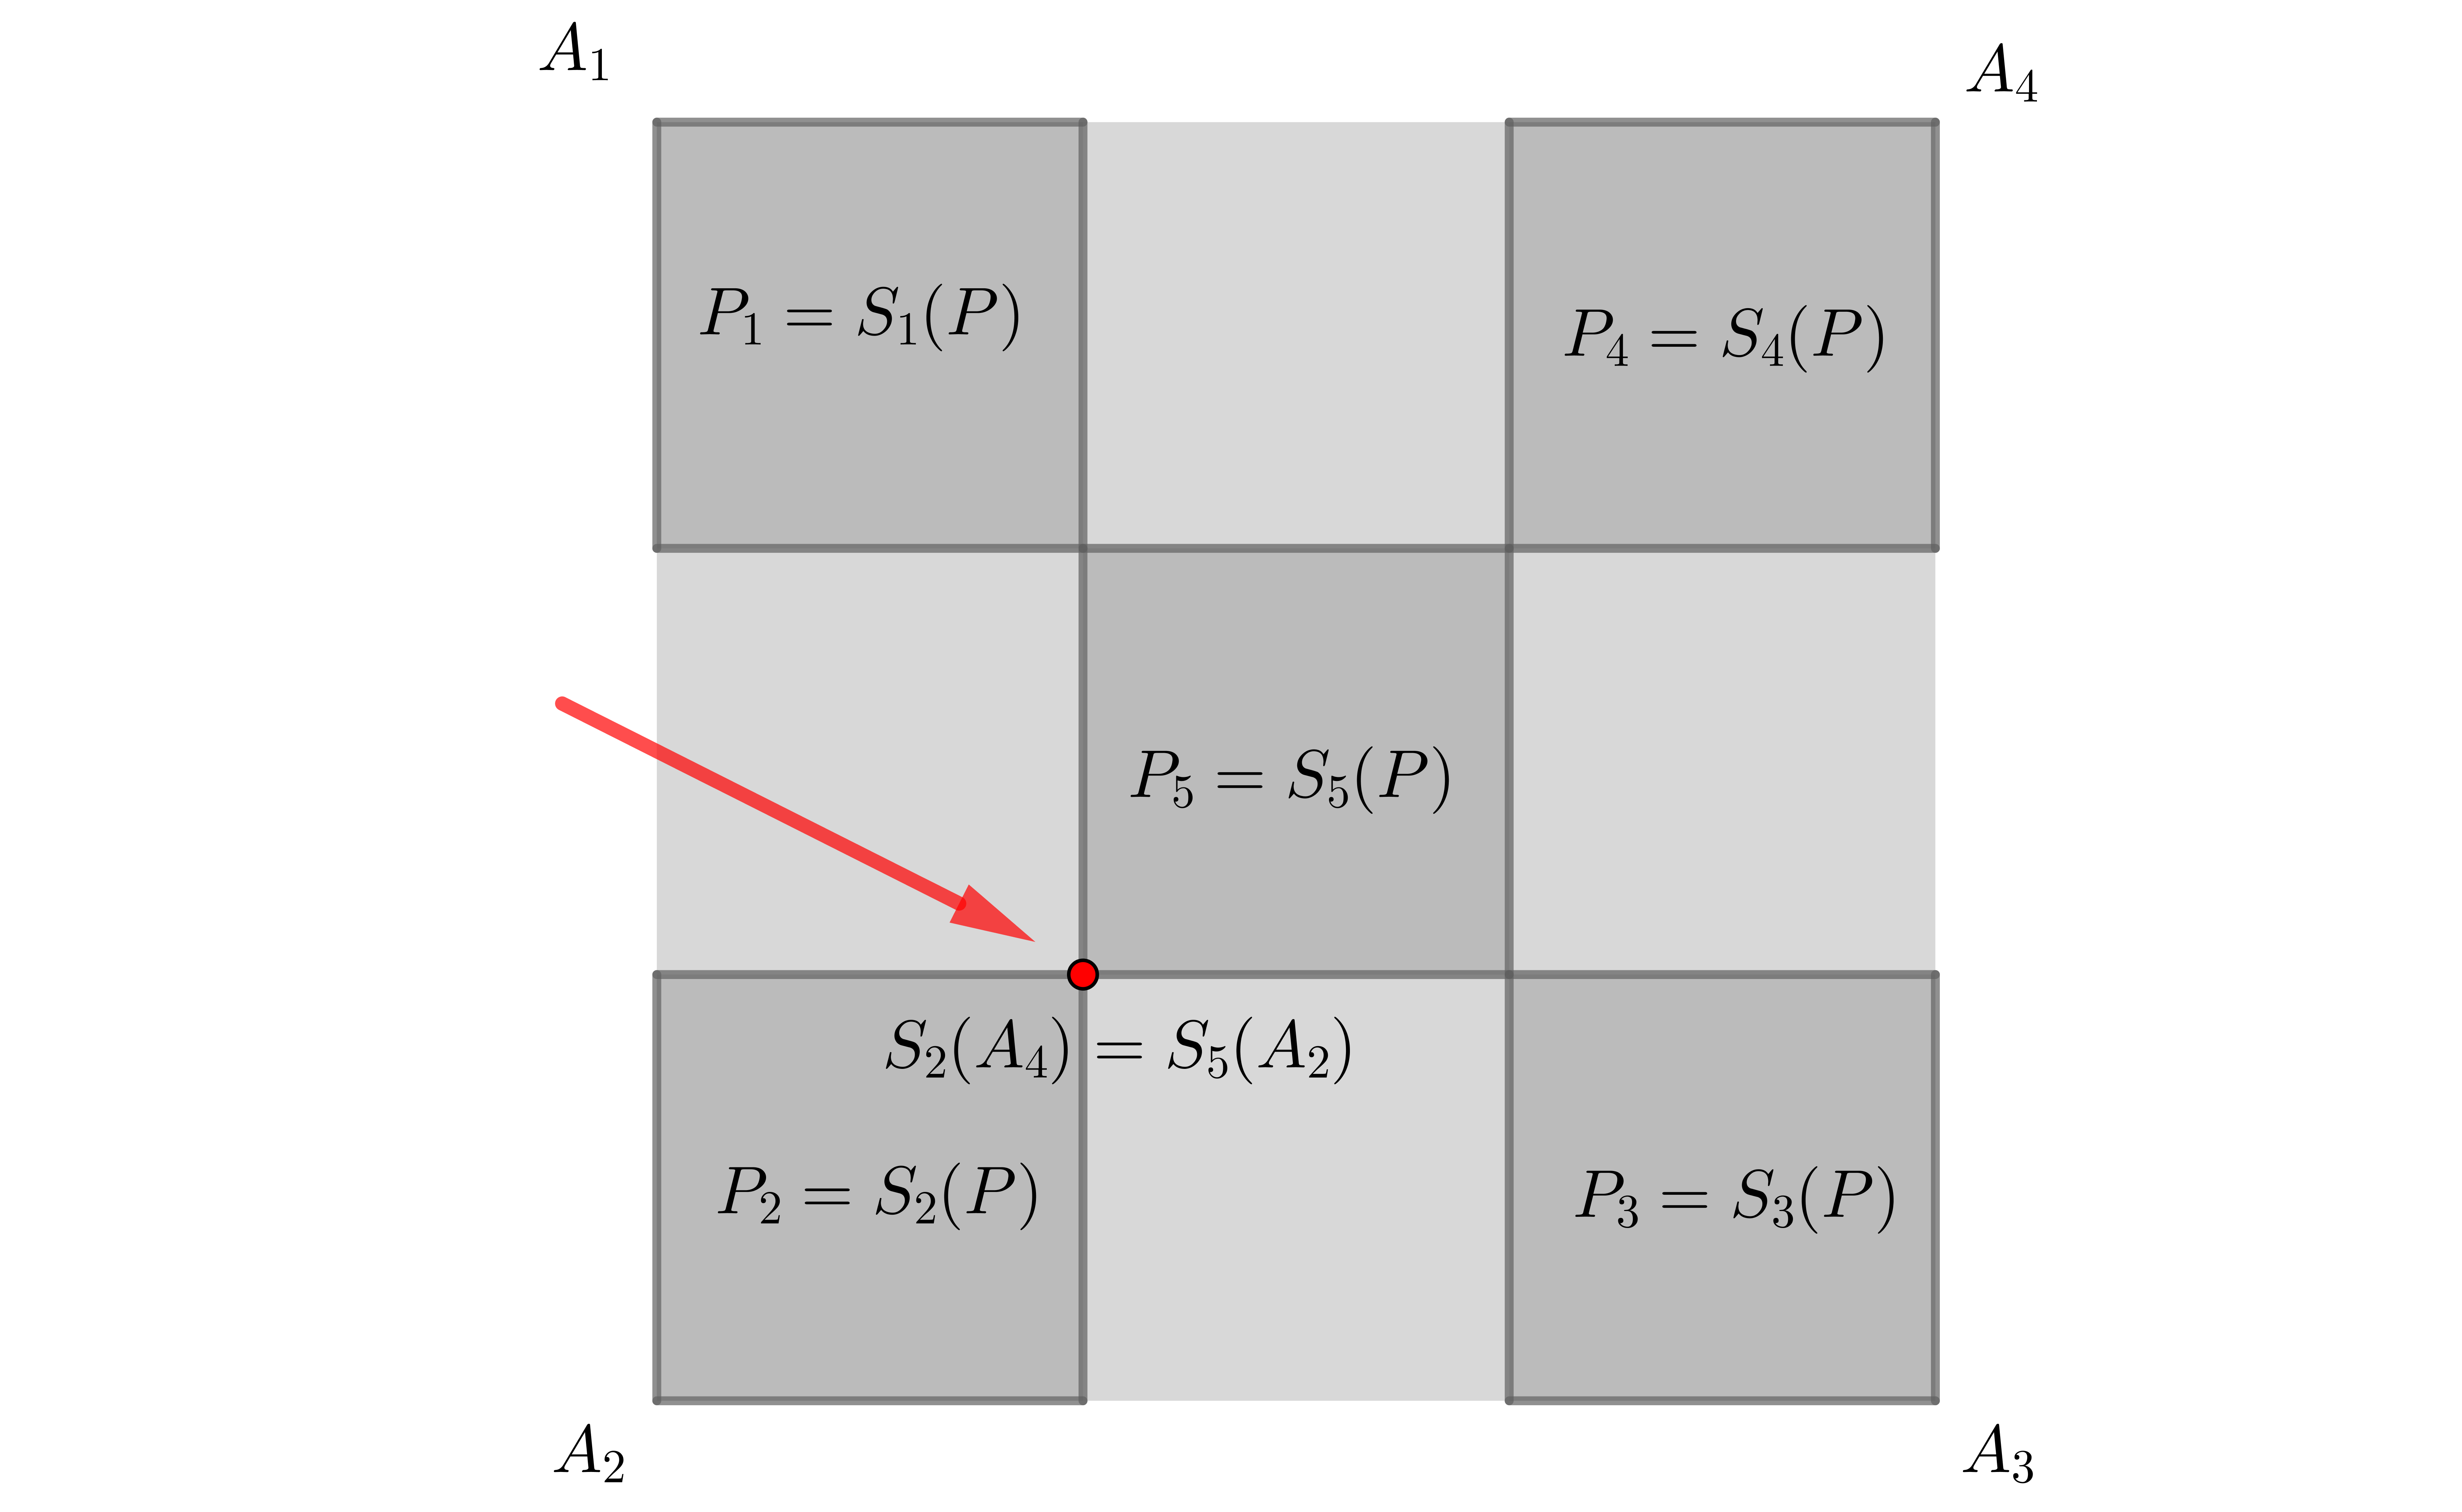
\includegraphics[width=.7\textwidth]{2_23.png}\]}
\only<4>{
{\bf(D1)}  для любого $i\in I$, множество $P_i=S_i(P)\IN P$;\\
{\bf(D2)}  для любых $i\neq j,\ \   i, j \in I,$ $P_i \cap P_j=V_{P_i}\cap V_{P_j}$ ;\\
{\bf(D3)}  $V_P\IN \bigcup\limits_{i\in I}S_i(V_P)$;\\
\[ 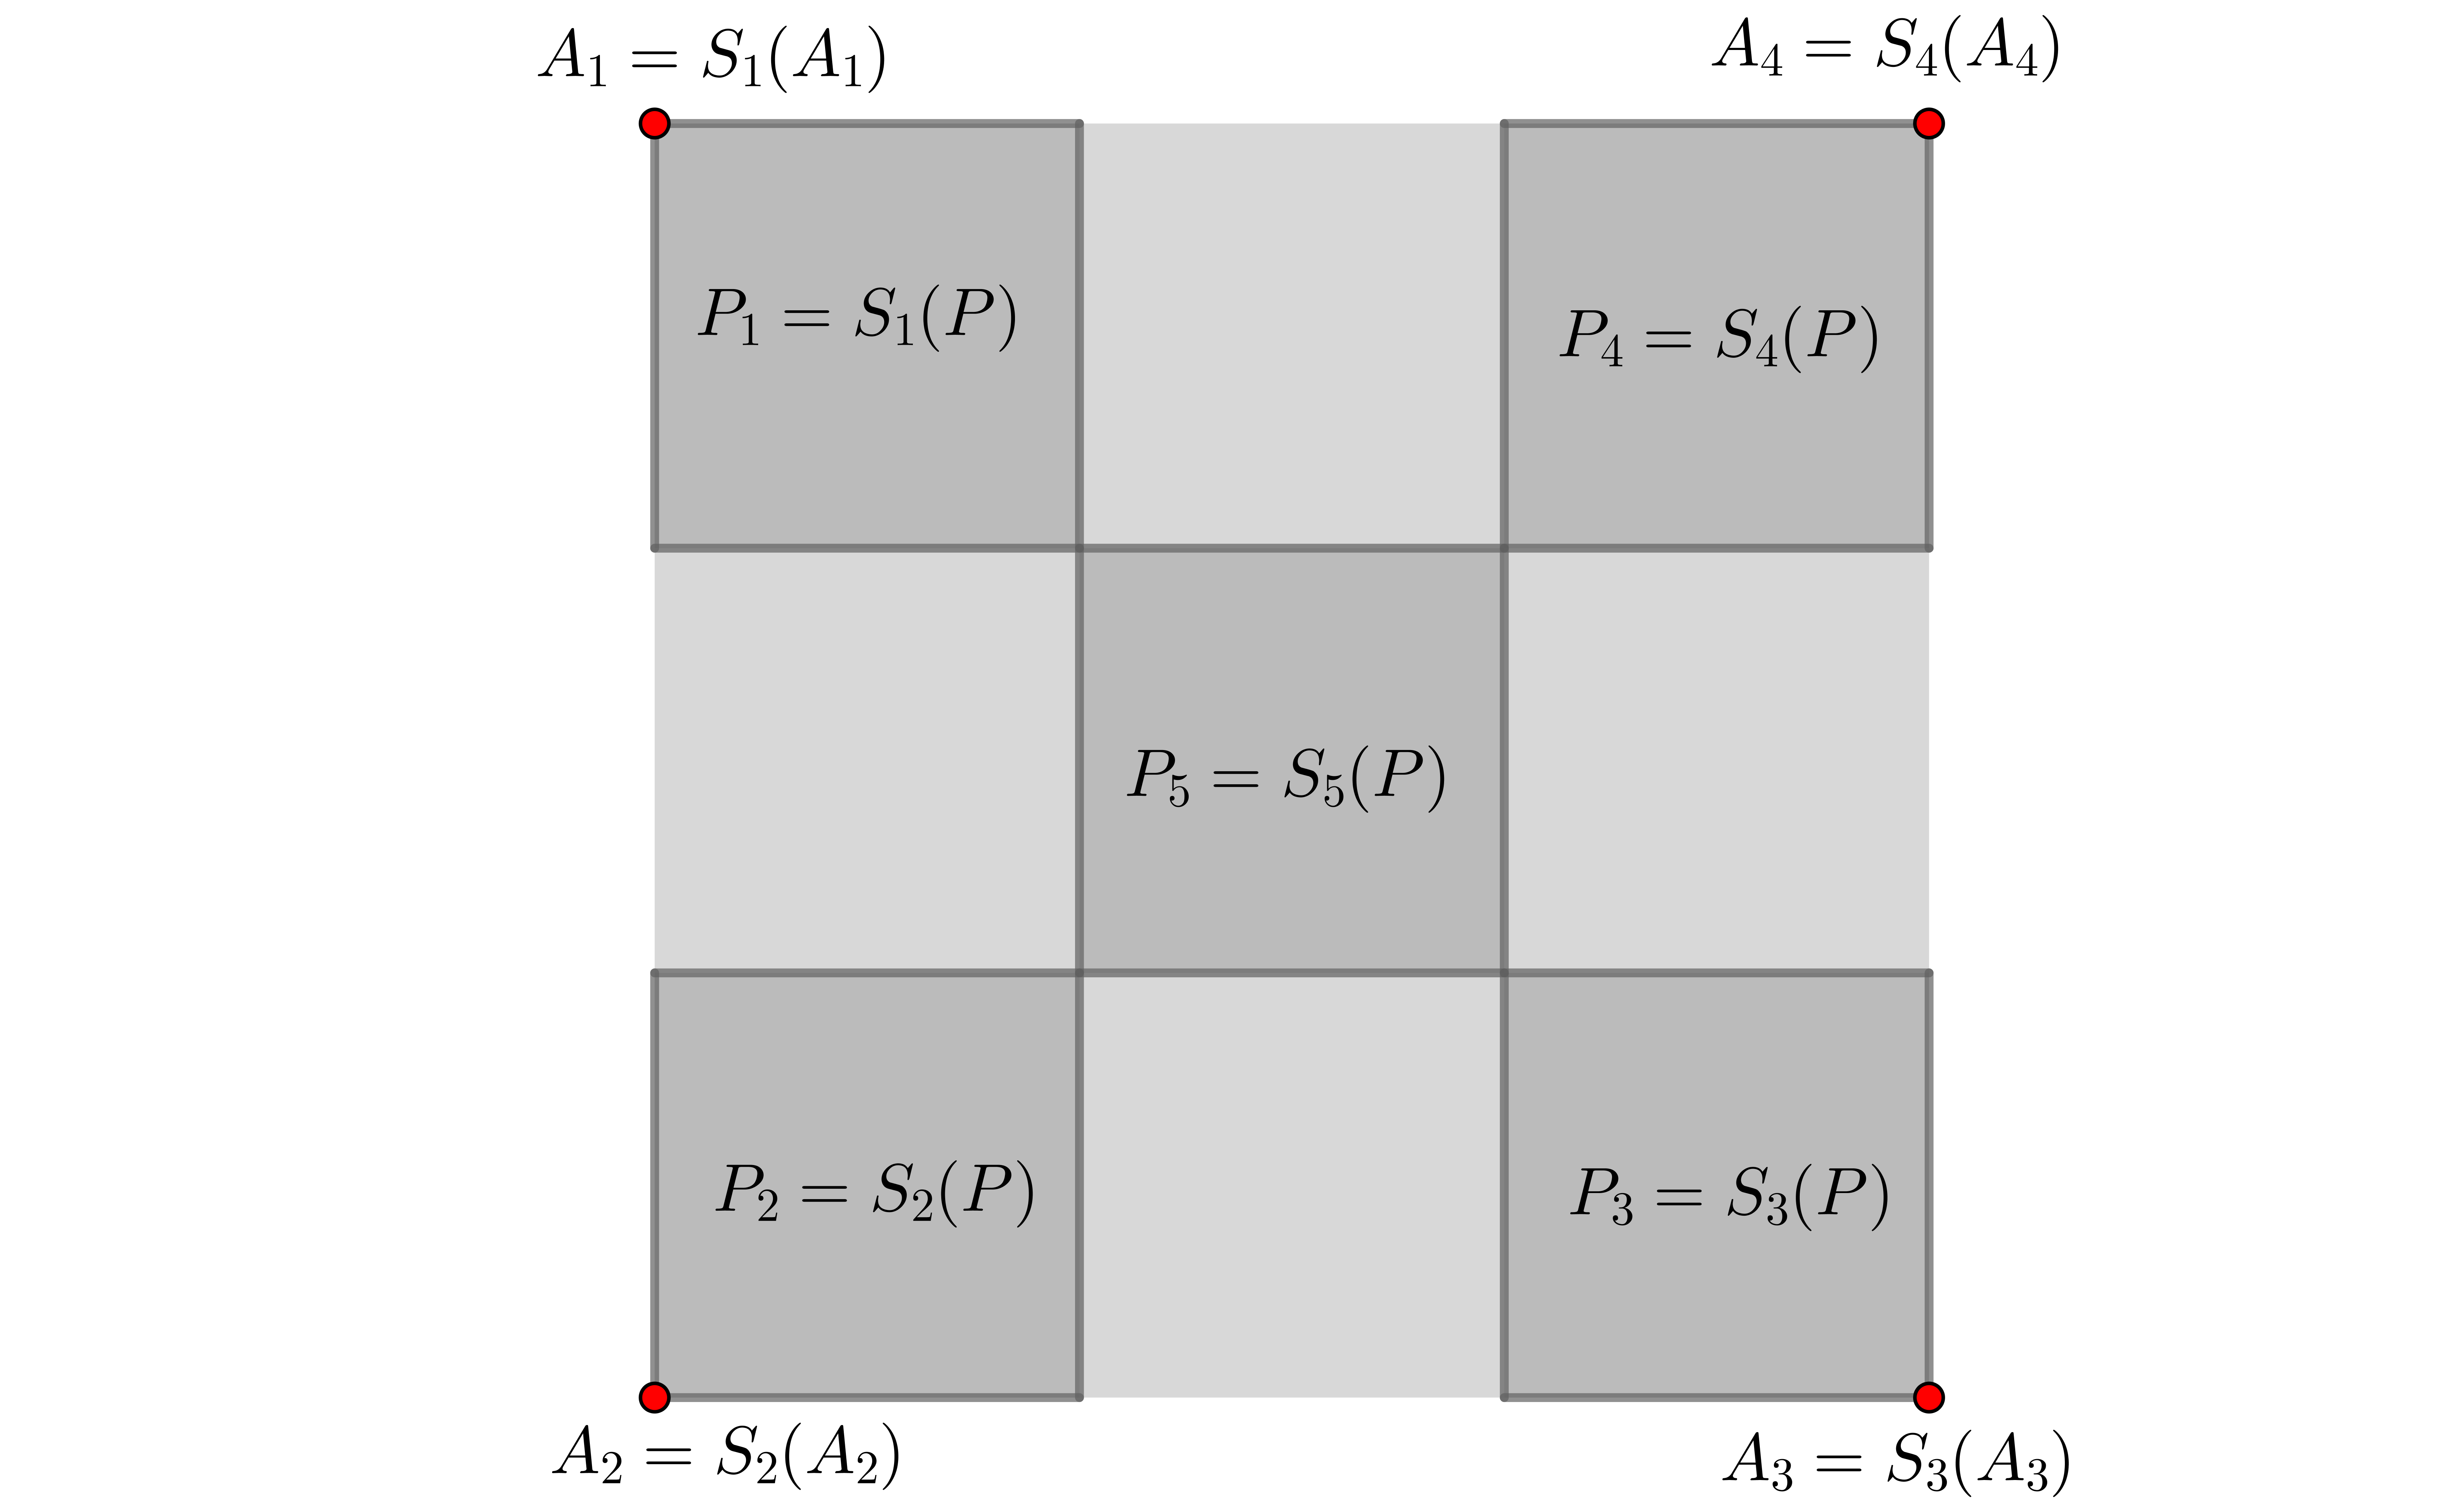
\includegraphics[width=.7\textwidth]{2_24.png}\]}
\only<5>{
{\bf(D1)}  для любого $i\in I$, множество $P_i=S_i(P)\IN P$;\\
{\bf(D2)}  для любых $i\neq j,\ \   i, j \in I,$ $P_i \cap P_j=V_{P_i}\cap V_{P_j}$ ;\\
{\bf(D3)}  $V_P\IN \bigcup\limits_{i\in I}S_i(V_P)$;\\
{\bf(D4)}  множество    ${\wP} = \bigcup \limits_{i = 1}^m P_i$ стягиваемо.
\begin{definition}
Система \ $\eS $, удовлетворяющая условиям {\bf (D1)-(D4)},
называется  стягиваемой $P$-полигональной  системой подобий.
\end{definition}
\begin{theorem} Аттрактор $K$  стягиваемой  $P$-полигональной  системы подобий $\eS$ является дендритом.
\end{theorem}}
\end{frame}


\begin{frame}{Примеры аттракторов стягиваемой полигональной системы}
\only<1>{
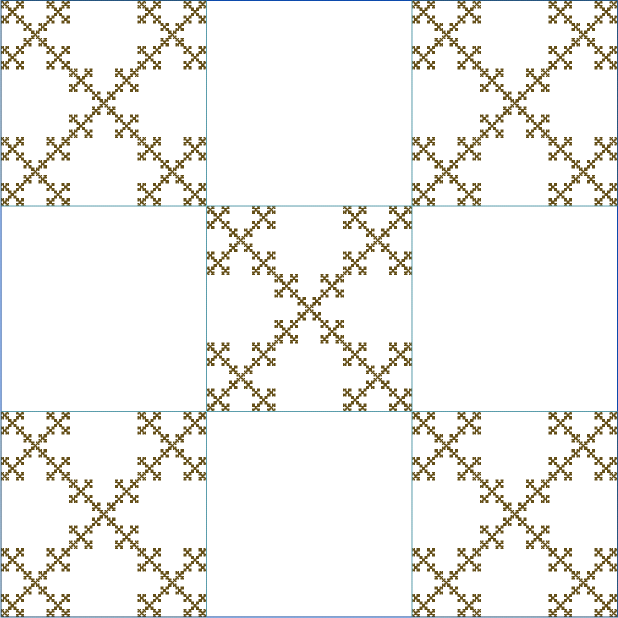
\includegraphics[width=0.44\textwidth]{14_7.png}
\hfill
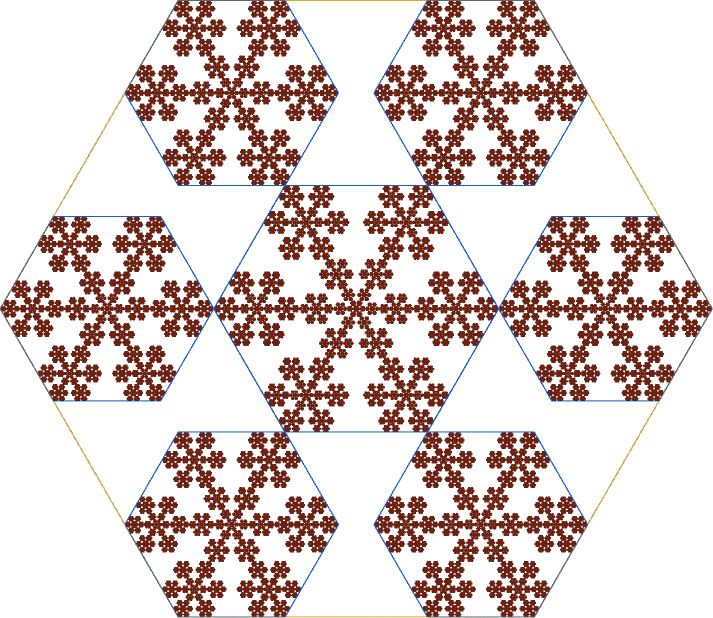
\includegraphics[width=0.5\textwidth]{14_6.png}}
\only<2>{
\begin{center}
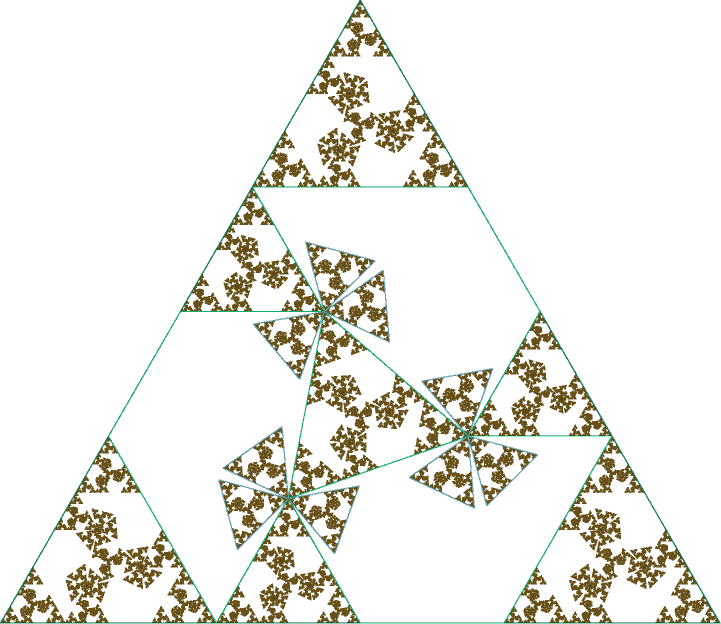
\includegraphics[width=0.7\textwidth]{14_5.png}
\end{center}}
\only<3>{
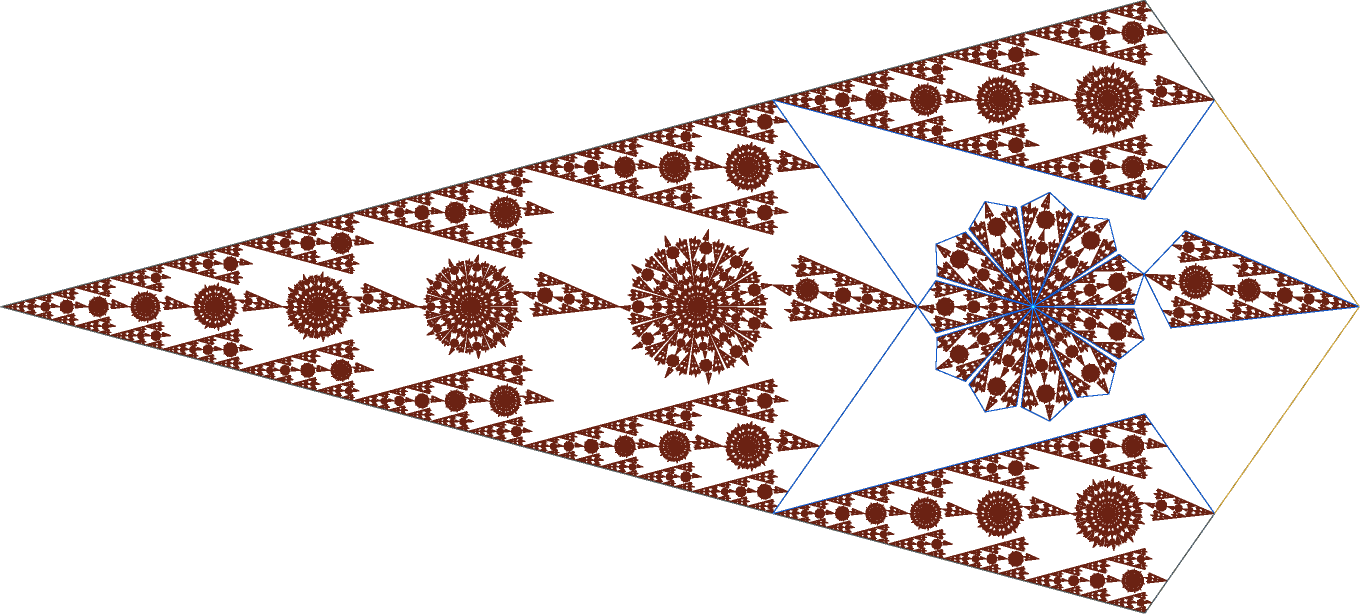
\includegraphics[width=1\textwidth]{14_4.png}}
\only<4>{
\begin{center}
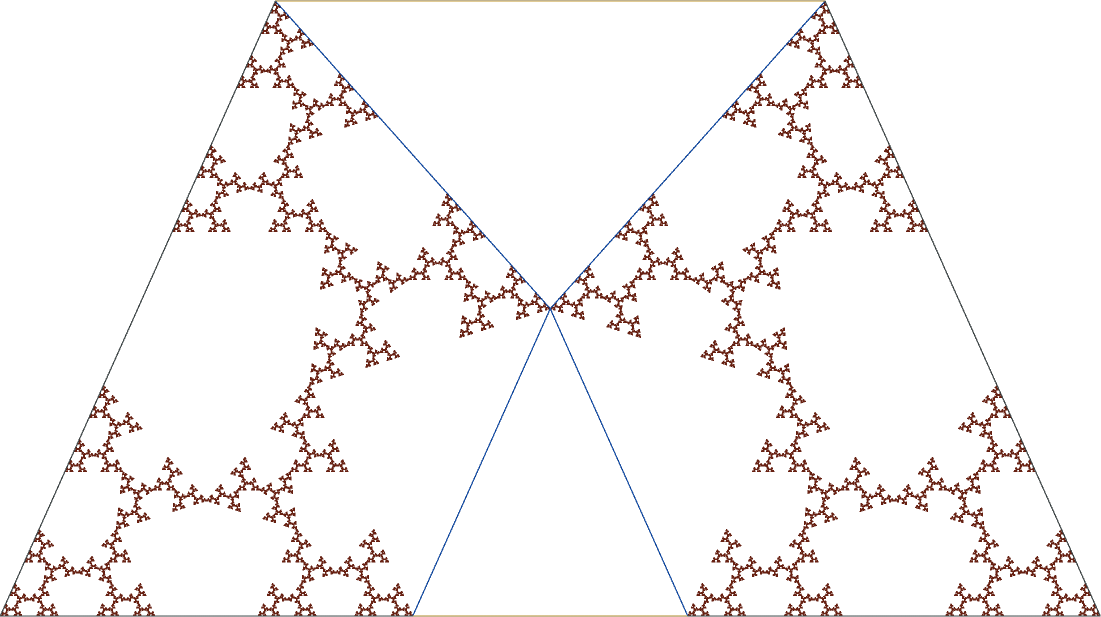
\includegraphics[width=0.5\textwidth]{14_1.png}
\hfill
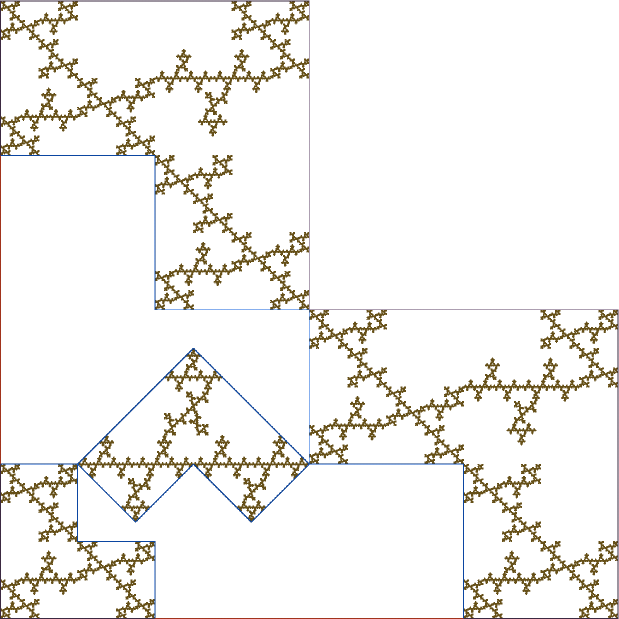
\includegraphics[width=0.4\textwidth]{14_3.png}
\end{center}}
\end{frame}


\begin{frame}{Обобщённая полигональная система}
\only<1>{
Даны многоугольник $P\IN \mathbb R^2$, множество его вершин $V_P=\{A_1,...,A_{n_P}\}$  и такая система подобий $\eS = \{S_1, \ldots, S_m\}$ в $\mathbb R^d$, что:\\
\textcolor[rgb]{0.75,0.75,0.75}{
{\bf(D1)}  для любого $i\in I$, множество $P_i=S_i(P)\IN P$;}\\
{\bf(D2)}  для любых $i\neq j,\ \   i, j \in I,$ $P_i \cap P_j=V_{P_i}\cap V_{P_j}$ ;\\
{\bf(D3)}  $V_P\IN \bigcup\limits_{i\in I}S_i(V_P)$;\\
{\bf(D4)}  множество    ${\wP} = \bigcup \limits_{i = 1}^m P_i$ стягиваемо.
\begin{definition}	
Если опустить условие {\bf (D1)}, то система \ $\eS $, удовлетворяющая условиям {\bf (D2)-(D4)},
называется  обобщённой $P$-полигональной  системой подобий.
\end{definition}}
\only<2>{
\begin{center}
%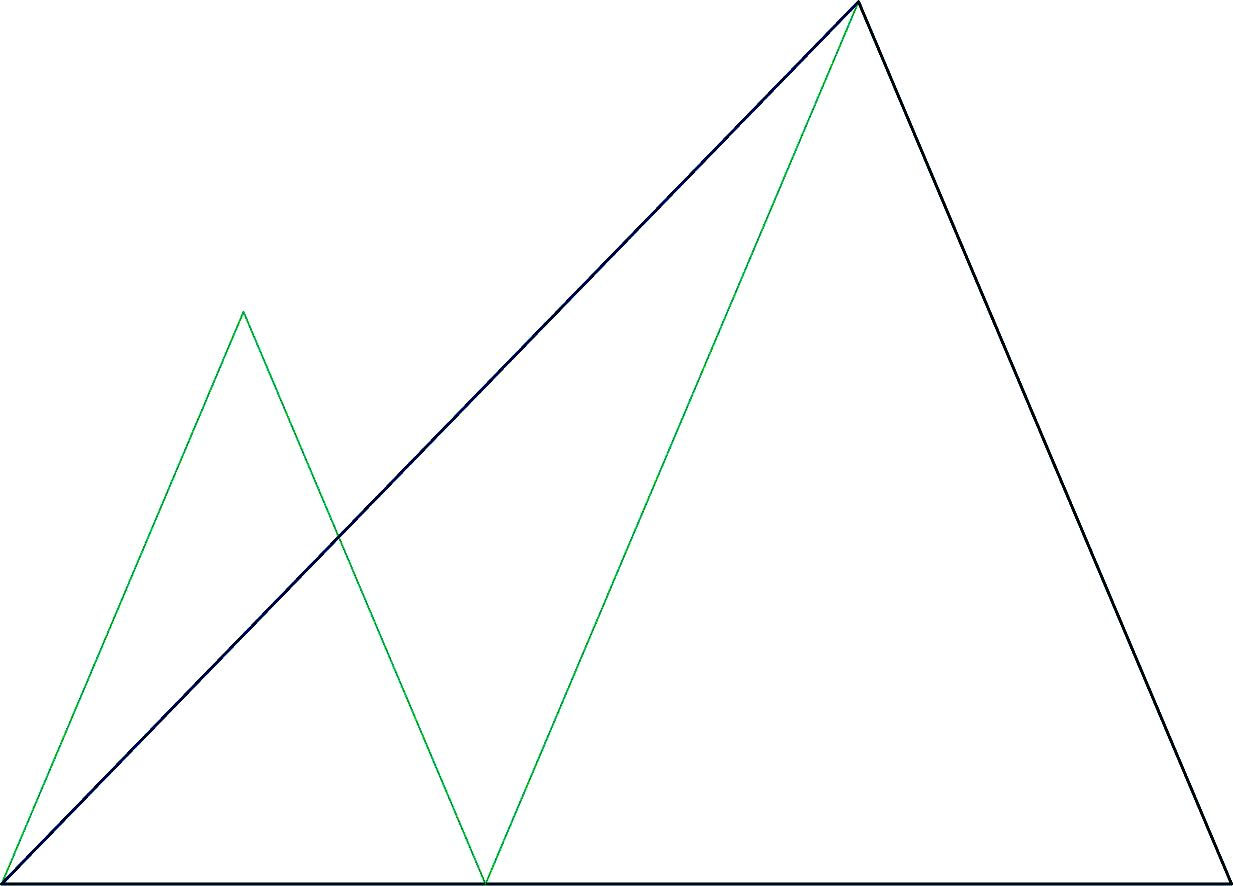
\includegraphics[width=0.45\textwidth]{pictures/gps1.jpg}
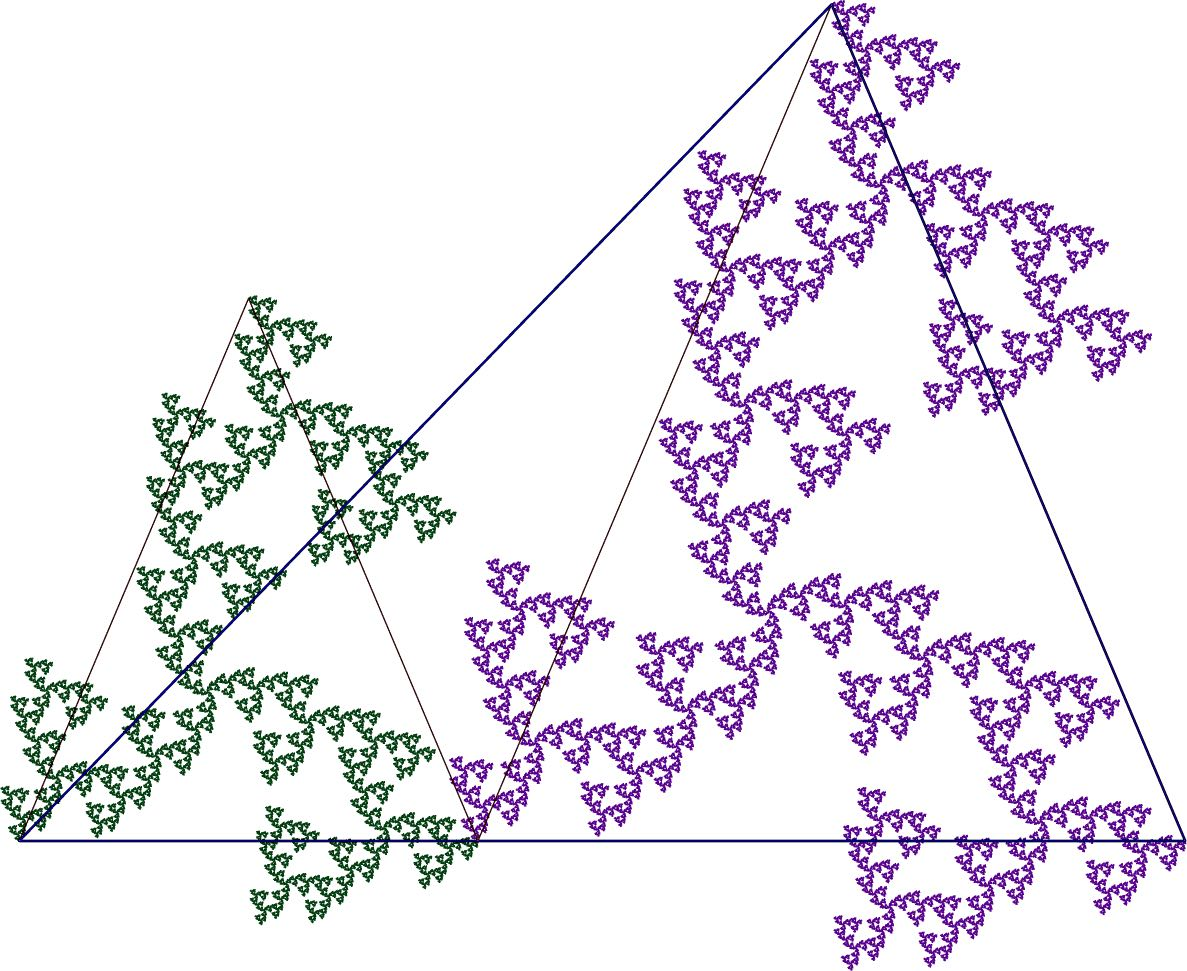
\includegraphics[width=0.7\textwidth]{tyl.jpg}
\end{center}}
\end{frame}


\begin{frame}{Критерий дендритности обобщённой полигональной системы}
\begin{theorem}
Пусть $\eS$ --- обобщенная $P$-полигональная система.  
Если для любых $i, j \in I$ 
\begin{equation}\label{icnd}S_i(K)\cap S_j(K)=P_i\cap P_j,\end{equation}
то аттрактор $K$ системы $\eS$ является дендритом.
\end{theorem}
\end{frame}


\begin{frame}{Дендрит с неодноточечным пересечением}
\begin{remark} 
Обобщенная $P$-полигональная система $\eS$ может не удовлетворять условию критерию дендритности и иметь аттрактор $K$, являющийся дендритом.
\end{remark}
\vfill
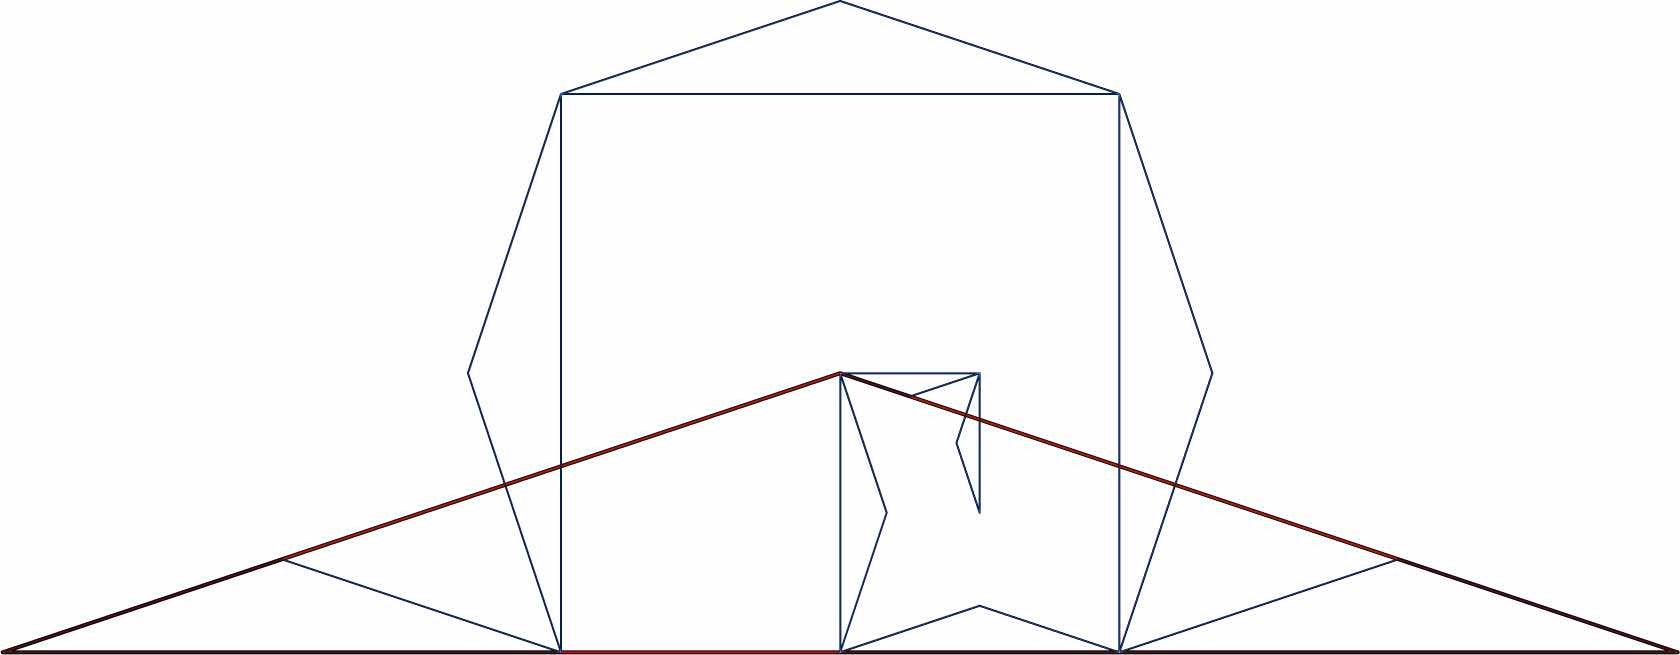
\includegraphics[width=.45\textwidth]{cntrex0.jpg}
\hfill
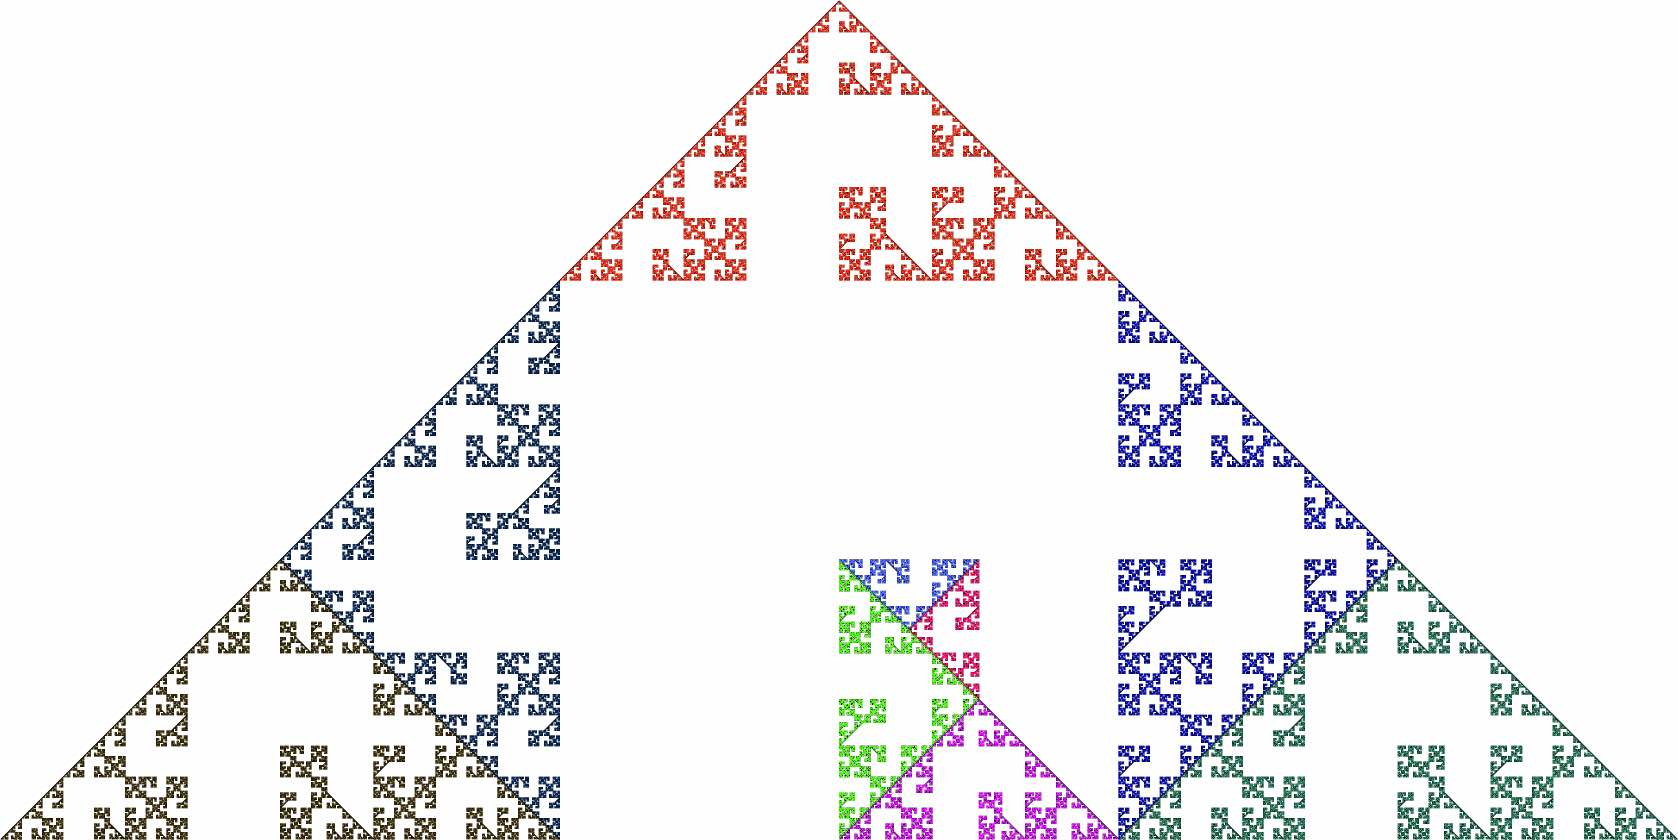
\includegraphics[width=.45\textwidth]{cntrex.jpg} 
\end{frame}


\begin{frame}{$\delta$-деформация}
\begin{definition}
Пусть $\delta>0$. 
Обобщенная $P'$-полигональная система $\eS'=\{S'_1,...,S'_m\}$ называется $\delta$-деформацией $P$-полигональной системы $\eS=\{S_1,...,S_m\}$, если существует биекция $f:\bigcup\limits_{k=1}^m \eV_{P_k}\to \bigcup\limits_{k=1}^m \eV_{P'_k}$ такая, что\\
a) $f|_{\eV_P}$ продолжается до гомеоморфизма $\tilde f: P\to  P'$; \\ 
b) $|f(x)-x|<\delta$  для любого $x\in \bigcup\limits_{k=1}^m \eV_{P_k}$\\  
c) $f(S_k(x))=S'_k(f(x))$ для любого $k\in I$ и $x\in \eV_P$.
\end{definition}
\end{frame}


\begin{frame}{Примеры аттракторов $\delta$-деформаций}
\only<1>{
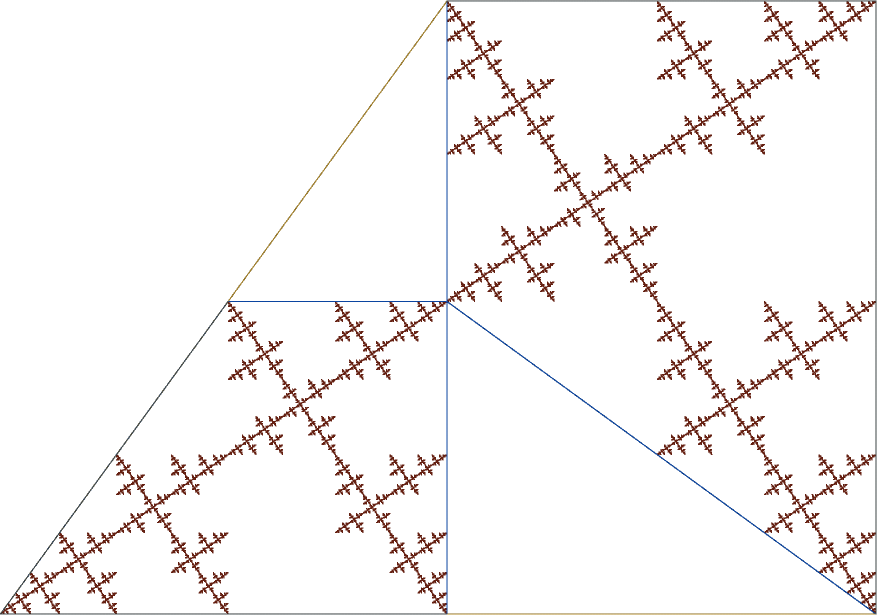
\includegraphics[width=0.45\textwidth]{14_2.png}
\hfill
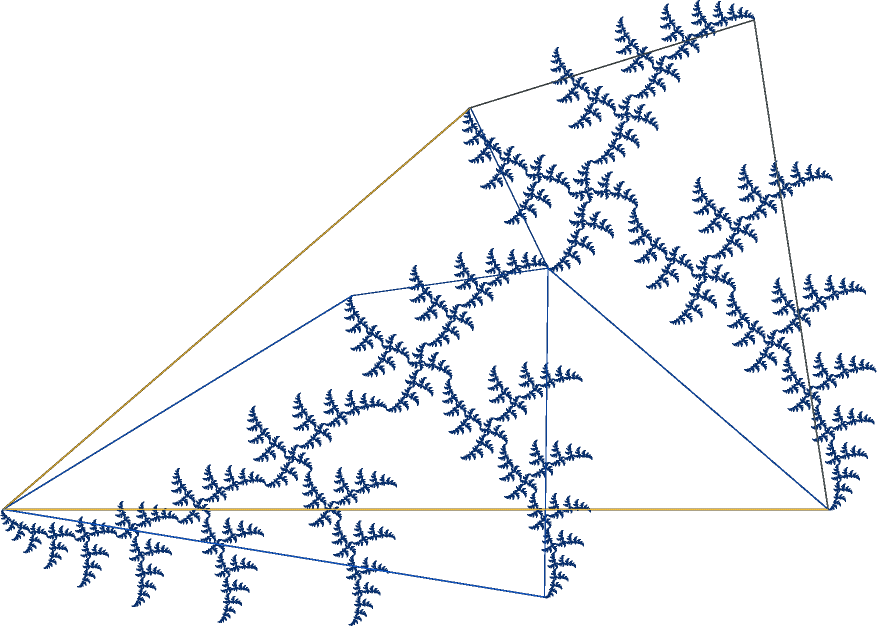
\includegraphics[width=0.45\textwidth]{2_14.png}}
\only<2>{
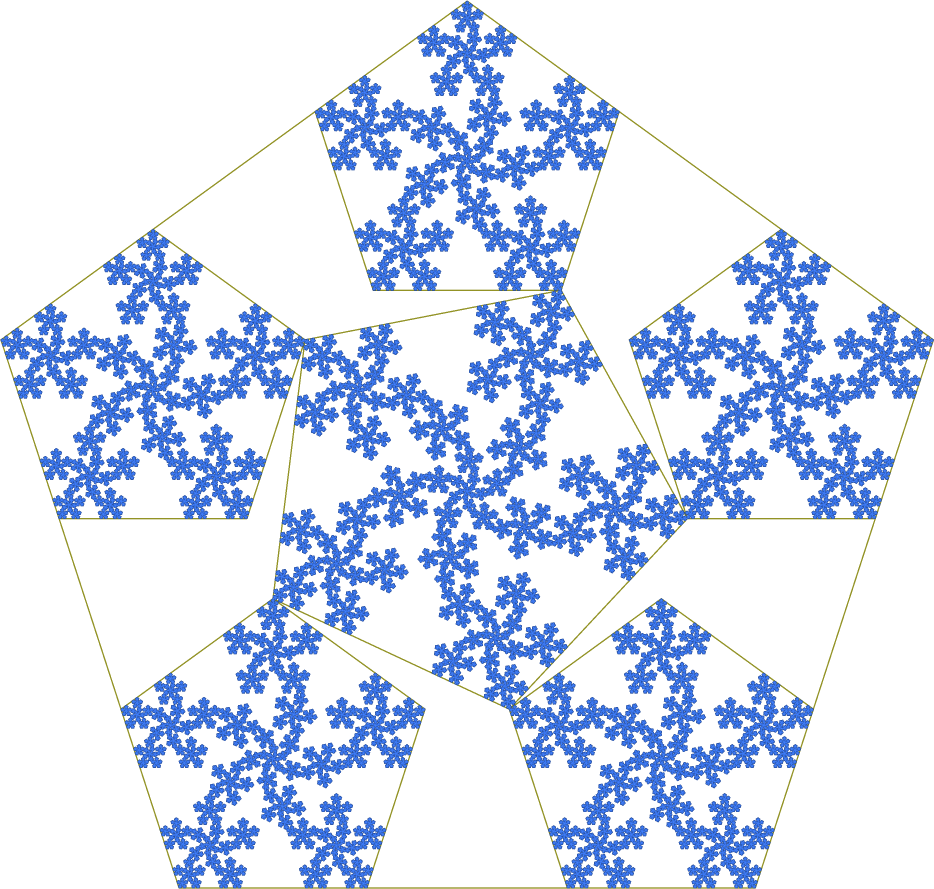
\includegraphics[width=0.45\textwidth]{5sps.png}
\hfill
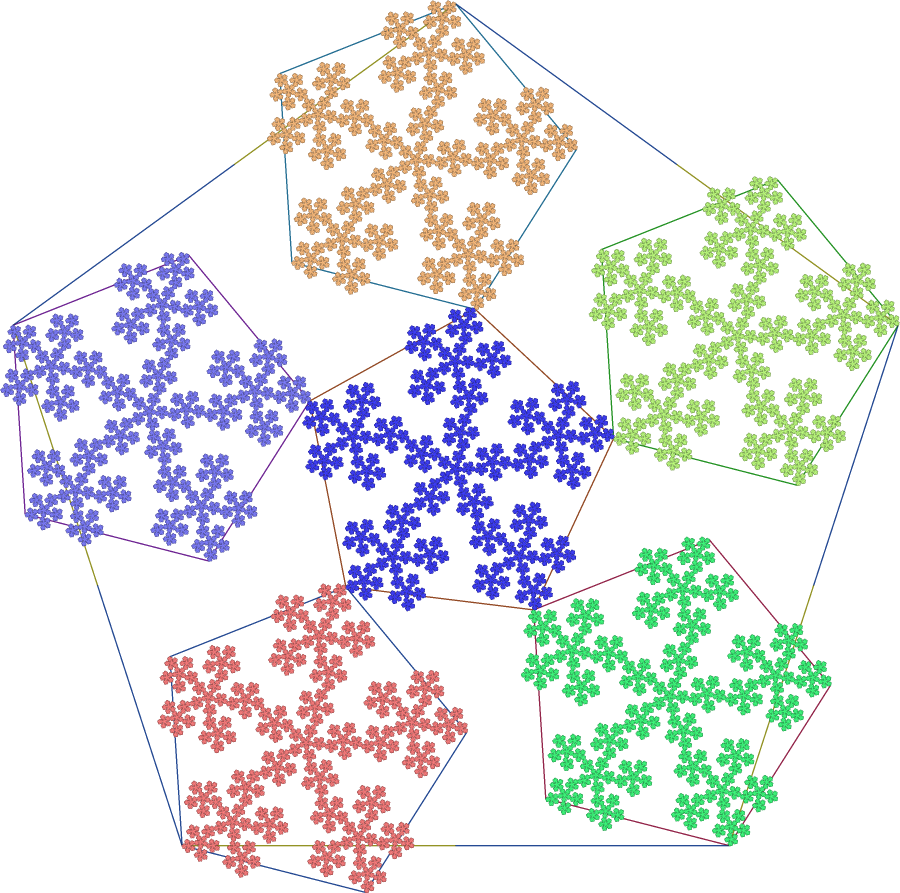
\includegraphics[width=0.45\textwidth]{5def.png}}
\only<3>{
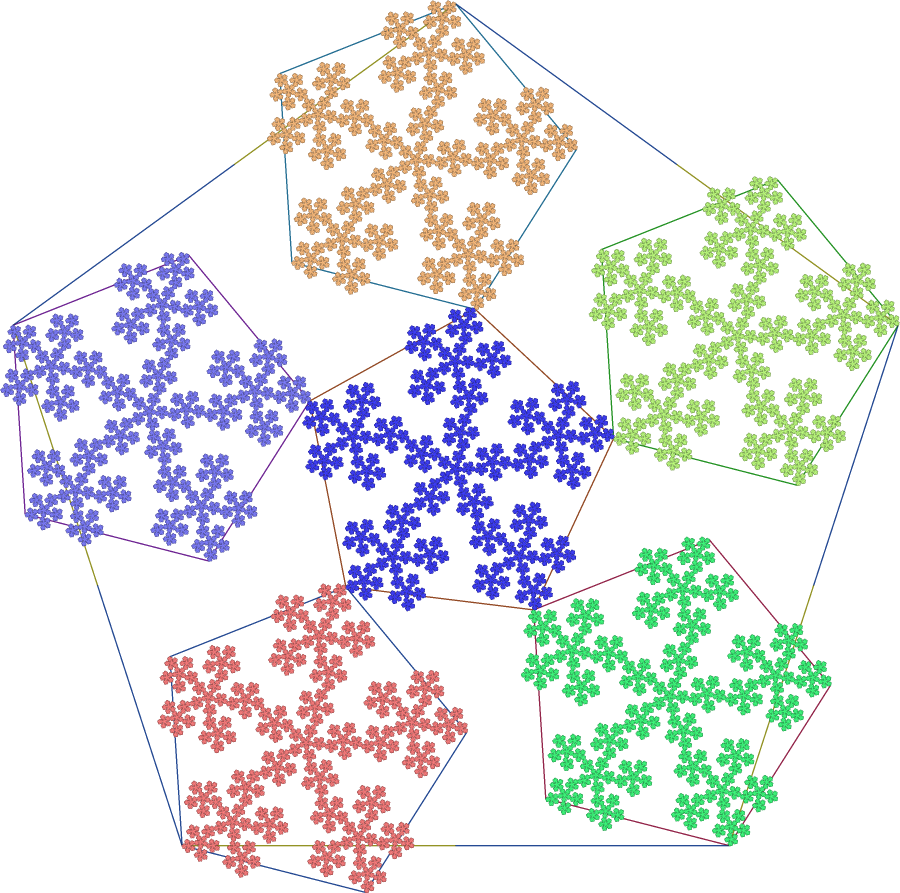
\includegraphics[width=0.45\textwidth]{5def.png}
\hfill
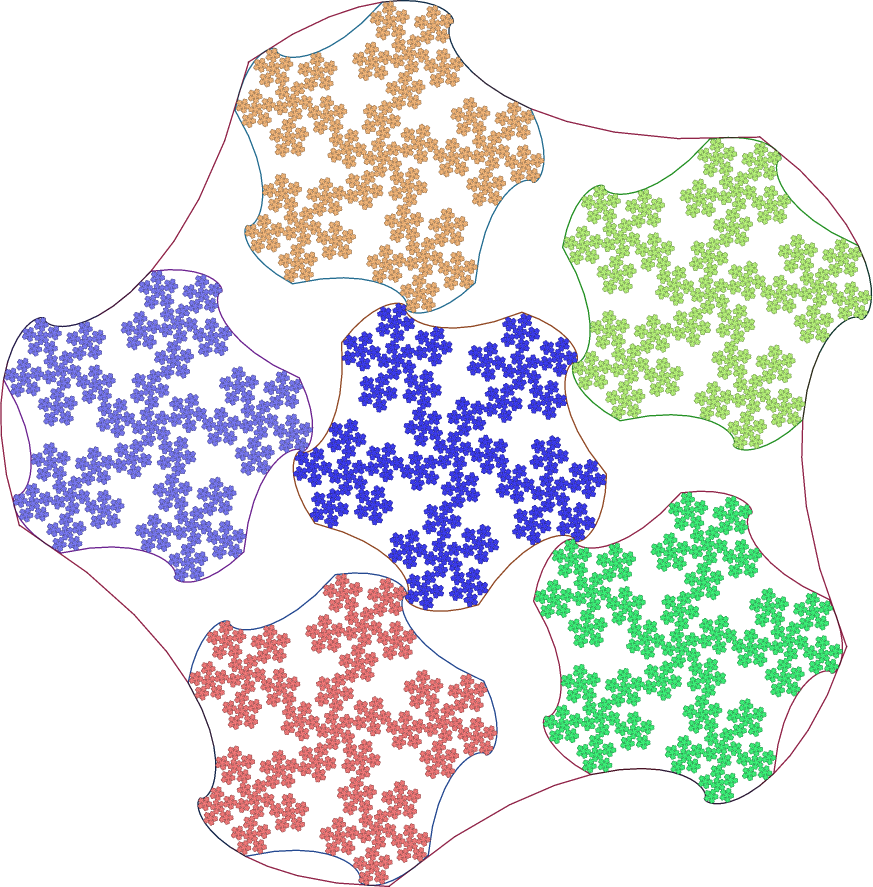
\includegraphics[width=0.45\textwidth]{5lox.png}}
\end{frame}


\begin{frame}{Циклические вершины и параметр вершины}
\begin{definition}
Пусть $\eS$ --- обобщенная $P$-полигональная  система подобий. Вершина $A \subset V_P$ называется циклической, если существует такой мультииндекс  $\bi=i_1 i_2 \ldots i_k$, что $S_\bi(A)=A$. Наименьшее из чисел $k=|\bi|$ по всем мультииндексам $\bi$ для которых $S_\bi(A)=A$ называется порядком циклической вершины $A$.
\end{definition}

\begin{definition}
Точка $B \in\cup_{i=1}^m  V_{P_i}$ подчинена циклической вершине $A$, если для некоторого мультииндекса $\bi, S_{\bi}(A)=B$.
\end{definition}

\begin{definition}
Если $S_i(z)=r e^{i \varphi} (z-A)+A$, то параметром $\lambda _A$ вершины $A$ называется число $\frac{\varphi}{\ln{r}}$, где угол $\varphi$ определяется геометрической конфигурацией системы.
\end{definition}
\end{frame}

\begin{frame}{}
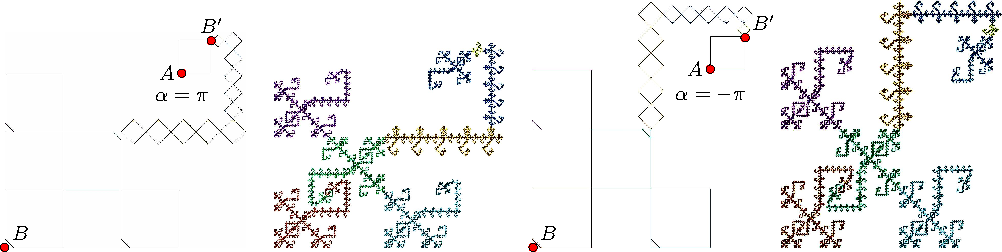
\includegraphics[width=\textwidth]{superden.pdf}
\end{frame}

\begin{frame}{Теорема о совпадении параметров}
\begin{block}{Условие совпадения параметров}
Для любых $B \in\cup_{i=1}^m  V_{P_i}$ и $A,A'$ таких, что, $S_i(A)=S_j(A')=B$, выполняется равенство $\lambda _i=\lambda _j$.
\end{block}
\begin{theorem}
Пусть обобщенная $P'$-полигональная система является $\delta$-деформацией некоторой стягиваемой $P$-полигональной системы $\eS$ и ее аттрактор $K'$ является дендритом. Тогда система $\eS$ удовлетворяет условию совпадения параметров.
\end{theorem}
\end{frame}

\begin{frame}{Индексная диаграмма}
\begin{definition}
Пусть $\eS=\{S_1,\ldots,S_m\}$ -- обобщенная $P$-полигональная система, аттрактор $K$ которой -- дендрит. Пусть $\eV=\{v_1,\ldots,v_n\}$ -- множество вершин многоугольника $P$. Индексной диаграммой мы назовем ориентированный граф $D=(\eV,E)$, для которого дуга $(v_i,v_j)\in E$ тогда и только тогда, когда существует такое $S_k\in\eS$, что $v_i=S_k(v_j)$. 
\end{definition}

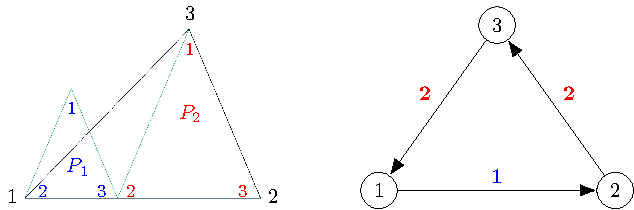
\includegraphics[width=\textwidth]{id1.pdf}

\end{frame}

\begin{frame}{Пример полигональной системы и её индексная диаграмма}
\only<1>{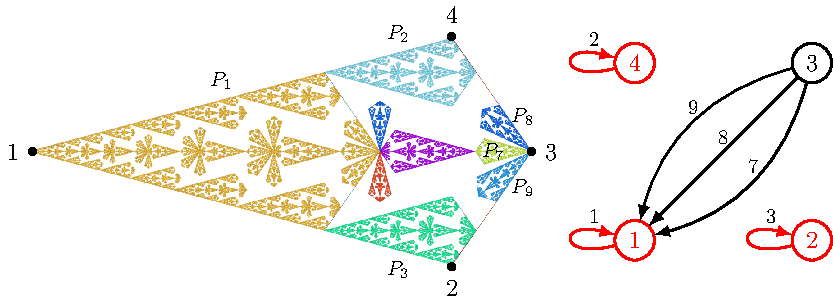
\includegraphics[width=\textwidth]{id3.pdf}}
\only<2>{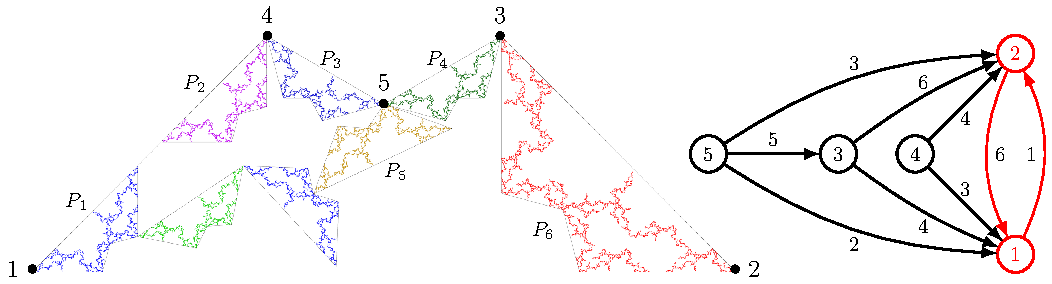
\includegraphics[width=\textwidth]{id4.pdf}}
\end{frame}


\begin{frame}{Теорема о малых деформациях}
\begin{theorem}
Для каждой полигональной системы $\eS$ существует такое $\delta > 0$, что для всякой $\delta$-деформации $S'$ полигональной системы $\eS$, удовлетворяющей условию совпадения параметров, аттрактор $K(\eS')$ является дендритом, гомеоморфным $K(\eS)$.
\end{theorem}
% 1)$\da<\dfrac{q_{min}}{8};$  
% 2)$\da<\dfrac{(1-q_{max})}{8};$ 
% 3)$\da<\dfrac{\rho_0}{2(C_k+1)};$ 
% 4)$\da<\dfrac{\rho_1}{4(C_k+1)};$ 
% 5)$\da<\dfrac{1-\rho_2}{2(C_k+1)};$ 
% 6)$\da<\dfrac{\al_0}{\dfrac{2.1(C_k+1)}{\rho_1}+C_{\la}\log (\dfrac{1+3\rho_2}{3\rho_1})},$\\
% где $C_\al=2.1(1+1/q_{min}), C_K=\dfrac{28+4C_\al}{1-q_{max}}$, а $C_\la=\dfrac{2.1(1+1/q_{max})}{\log(3+q_{max})-\log(3q_{max}+1)}.$ 
\end{frame}


\begin{frame}{}
\Huge{Часть 2.\\
Пересечения фрактальных кубов}
\end{frame}



\begin{frame}{Актуальность}
\begin{thebibliography}{9}
\footnotesize{

\bibitem{bedf1984}    
	{\sc Bedford, T.}
    {\it Crinkly curves, Markov partitions and dimension.}
    Ph.D. thesis, University of Warwick, 1984.

\bibitem{McMul}    
	{\sc McMullen, C.}
	{The {Hausdorff} dimension of general {Sierpi{\'n}ski} carpets.}
	{\it Nagoya Mathematical Journal 96} (1984), 1--9.

\bibitem{bib:peres1996}
    {\sc Kenyon R., Peres Y.,} 
    {\em Measures of full dimension on affine-invariant sets,}
    {Ergod. Th. \& Dynam. Sys. (2) \textbf{16} (1996), 307--323}

\bibitem{bib:peres1994}
    {\sc Peres Y.,}
    {\em The self-affine carpets of McMullen and Bedford have infinite Hausdorff measure,}
    {Math. Proc. Camb. Phil. Soc. (3) \textbf{116} (1994), 513--526}

%\bibitem{bib:Olsen1998}    
%    {\sc Olsen L.,}
%    {\em Self-affine multifractal Sierpinski sponges in $\rr^d$,}
%    {Pac. J. Math. \textbf{116} (1998), 143--199}

\bibitem{cristea2020}    
	{\sc Cristea, L. L. and Leobacher, G.}
	{Supermixed labyrinth fractals.}
	{\it Geometriae Dedicata 141}, 1 (2009), 1--17.

\bibitem{cristea2009}    
	{\sc Cristea, L. L. and Steinsky, B.}
	{Curves of infinite length in 4×4-labyrinth fractals.}
	{\it Geometriae Dedicata 141}, 1 (2009), 1--17.

\bibitem{cristea2011}    
	{\sc Cristea, L. L. and Steinsky, B.}
	{Curves of infinite length in labyrinth fractals.}
	{\it Proceedings of the Edinburgh Mathematical Society 54}, 2 (2011), 329--344.
	
\bibitem{cristea2017}    
	{\sc Cristea, L. L. and Steinsky, B.}
	{Mixed labyrinth fractals.}
	{\it Topology and its Applications 229} (2017), 112–125.

\bibitem{bib:LLR2013}    
    {\sc Lau K., Luo J.J.,Rao H.}
    {\em Topological structure of fractal squares,}
    {Math. Proc. Camb. Phil. Soc. \textbf{155} (2013), 73--86}
}

\bibitem{Xiao2021} 
	{\sc J.-C. Xiao,} 
	{\em Fractal squares with finitely many connected components,}
	{Nonlinearity, (4)\textbf{34} (2021) 1817–1836}
	
\bibitem{Fraser2021} 
	{\sc J. M. Fraser,}
	{Fractal Geometry of Bedford-McMullen Carpets,} 
	{in Thermodynamic Formalism, M. Pollicott and S. Vaienti, Eds., 
	Springer International Publishing (2021)}
\end{thebibliography}
\end{frame}


\begin{frame}{Цели и выносимые на защиту положения}
Цель:
\begin{enumerate}
\item[$\bullet$] Описать структуру пересечения фрактальных кубов;
\end{enumerate}

\hfill

Выносимые на защиту положения:
\begin{enumerate}
\item[1] Описана граф-ориентированная система подобий, компонентами которой являются как пересечение пары фрактальных кубов, так и пересечения их противоположных граней;
\item[2] Получены условия того, что пересечение будет конечным (в точ числе одноточечным);
\item[3] Получены условия того, что пересечение будет имеьь бесконечную меру.
\end{enumerate}
\end{frame}


\begin{frame}{Граф-ориентированная система}
\only<1>{
    \begin{definition}[Mauldin \& Williams (1988)]
        Пусть $\{\eS_{ij}\ |\ i,j=1,\ldots,k\}$ --- набор систем сжимающих отображений, причём для некоторых $i, j$ система $\eS_{ij}$ может быть пустой.
        Пусть этим системам соответствуют операторы Хатчинсона $\{T_{ij}(A)\}$.
        Тогда набор компактов
        $$\left\{K_i=\bigcup\limits_{j=1}^k T_{ij}(K_j)\ |\ i=1,\ldots,k\right\}$$ 
        будем называть аттрактором граф-ориентированной системы из $k$ компонент.
    \end{definition}
    \centering{
        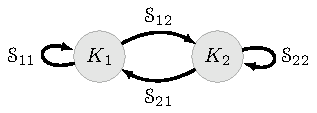
\includegraphics[width=0.5\textwidth]{GDS.pdf}}
    \footnotetext[2]{Mauldin R. D., Williams S. C., Hausdorff dimension in graph directed constructions, Trans. Amer. Math. Soc. (2) \textbf{309} (1988), 811--829.}}
\only<2>{
    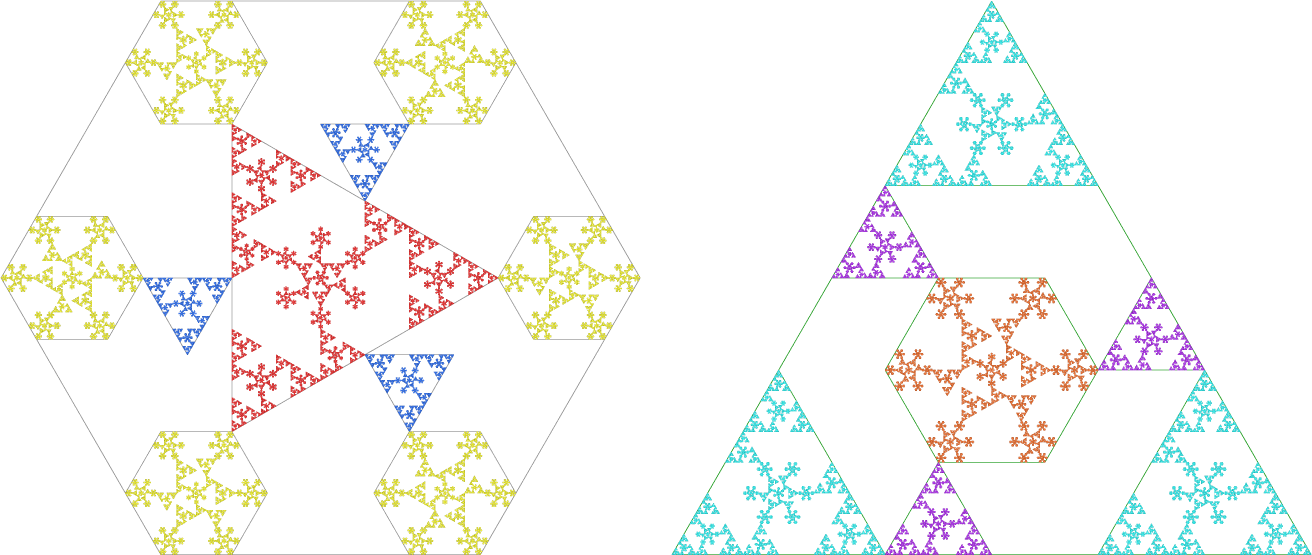
\includegraphics[width=\textwidth]{gds2.png}}
\end{frame}


\begin{frame}{
\only<1>{Фрактальный $k$-куб}
\only<2>{Фрактальный квадрат}
\only<3>{Фрактальный куб}
}
\only<1>{
    \begin{definition}[Olsen L. (1998); Lau K., Luo J.J.,Rao H. (2013)]
    Пусть  $D=\{d_1,\ldots,d_r\},\; d_i\in\{0,1,\ldots,n-1\}^k$, где $n\ge 2$, а $1<\#D<n^k$.\\
    {\em Фрактальным $k$-кубом}   порядка $n$  с {\em множеством единиц $D$} называют компактное множество $K\IN\rr^k$,  удовлетворяющее 
    $$K=\dfrac{K+D}{n}$$
    \end{definition} 
    \begin{remark}
    Фрактальный $k$-куб $K=\dfrac{K+D}{n}$ с множеством единиц $D=\{0,1,\ldots,n-1\}^k$ есть единичный $k$-мерный куб $P$.
    \end{remark}
    % \begin{corollary}
    % $K=\dfrac{K+D}{n}\IN P$
    % \end{corollary} 
    \footnotetext[3]{Olsen L., Self-affine multifractal Sierpinski sponges in $\rr^d$, Pac. J. Math. \textbf{116} (1998), 143--199}
    \footnotetext[4]{Lau K., Luo J.J.,Rao H., Topological structure of fractal squares, Math. Proc. Camb. Phil. Soc. 115 (2013), 73--86}
}
\only<2>{
    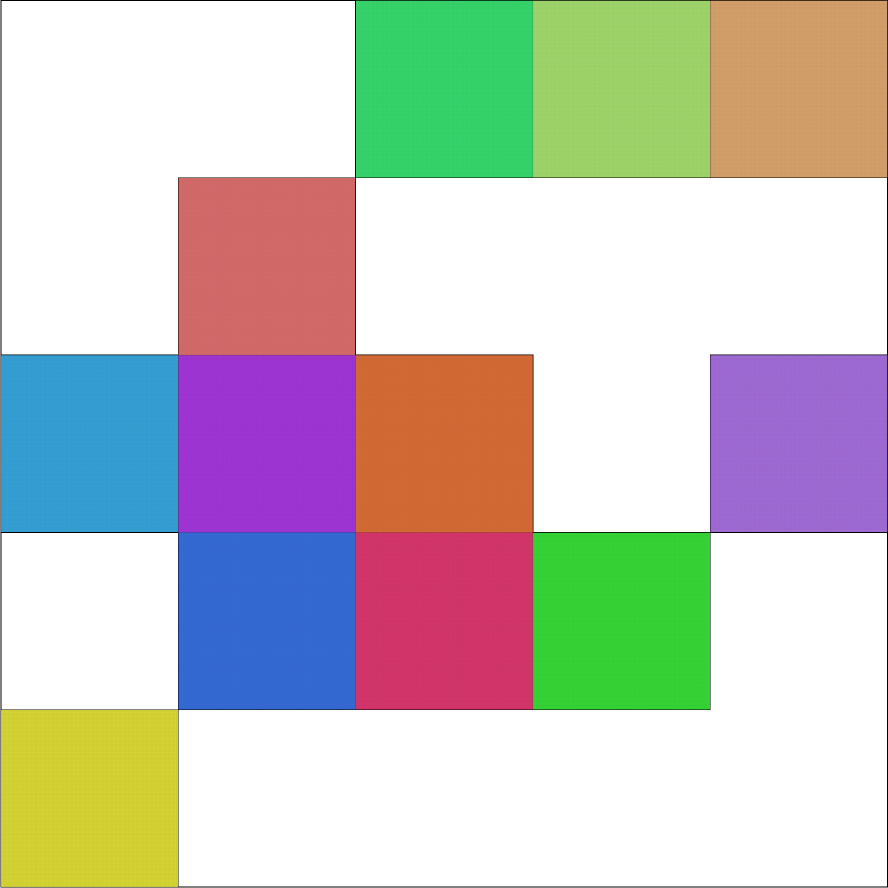
\includegraphics[width=0.45\textwidth]{den3f1.png}
    \hfill
    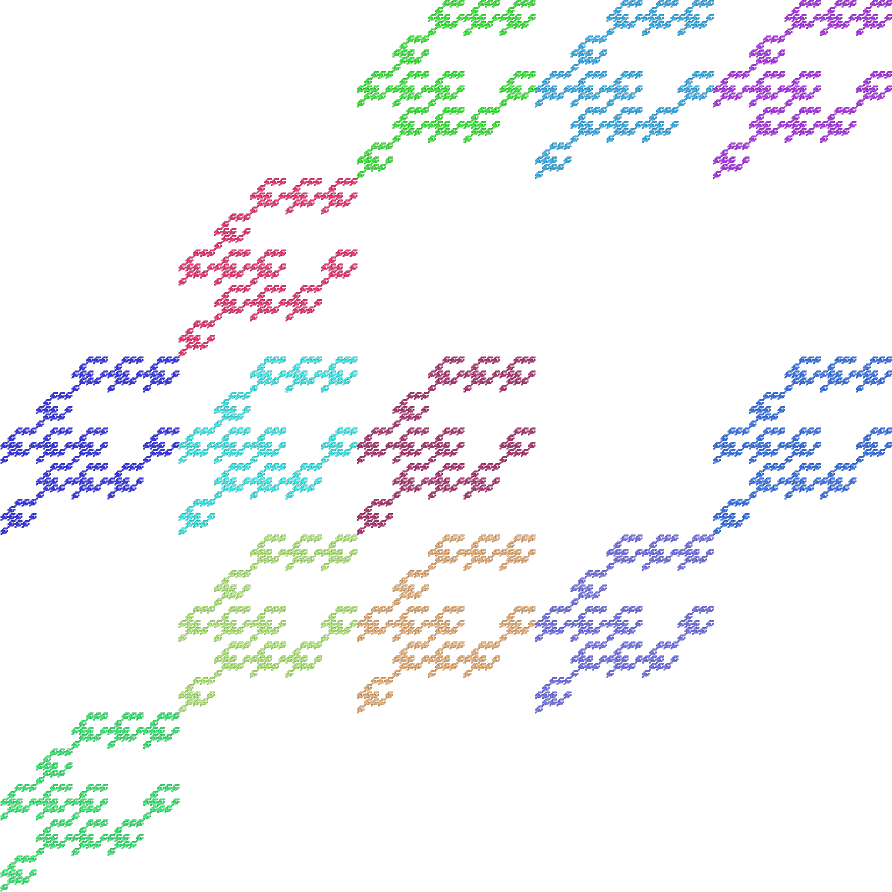
\includegraphics[width=0.45\textwidth]{den3f.png}
    % $$K=\dfrac{K+D}{n}=\bigcup_{i=1}^rS_i(K),\; \text{ где }\; S_i(x)=\frac{d_i+x}{n}\; \text{ и }\; \fix(S_i)=\frac{d_i}{n-1}.$$
    }
\only<3>{
    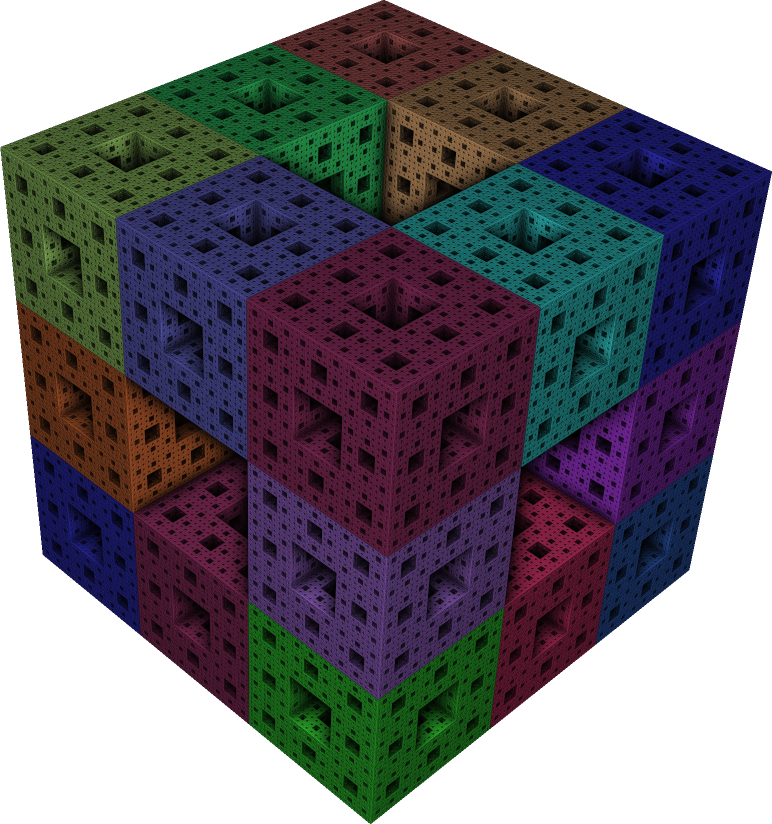
\includegraphics[width=0.45\textwidth]{menger_sponge_f.png}
    \hfill
    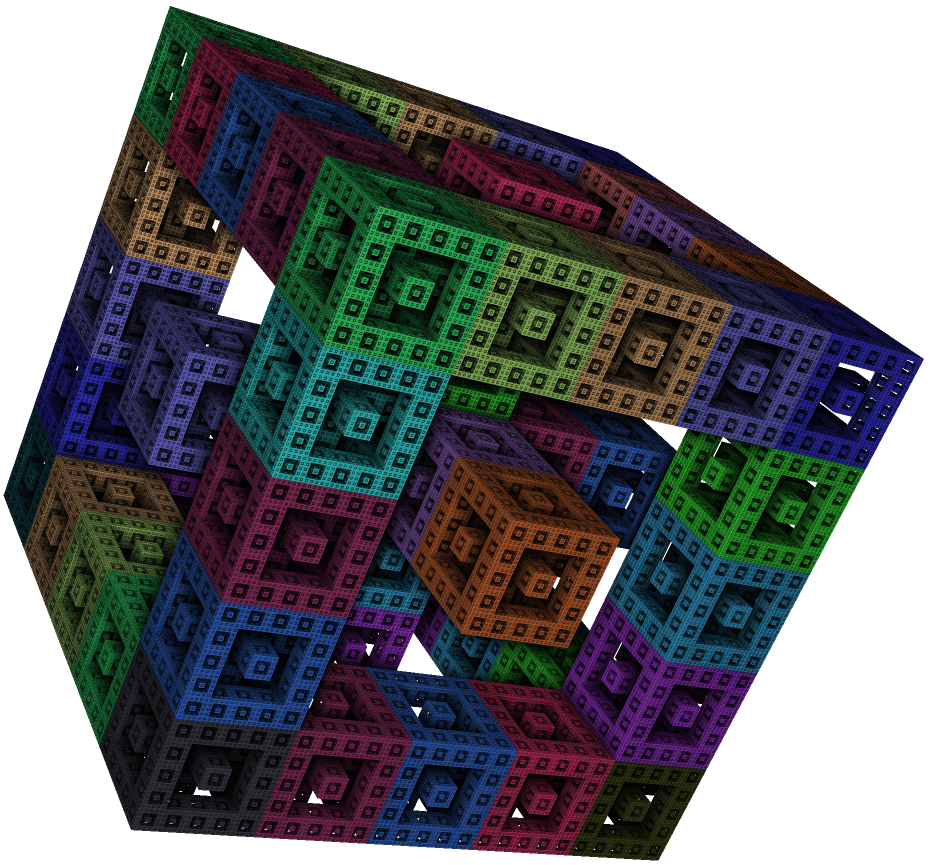
\includegraphics[width=0.5\textwidth]{Q555.png}}
\end{frame}


\begin{frame}{Грани единичного $k$-куба}
\begin{columns}
\column{0.5\textwidth}
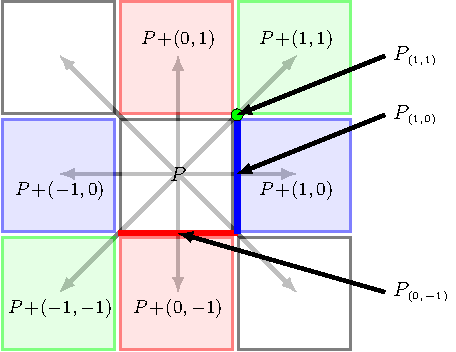
\includegraphics[width=\textwidth]{presentation/faces.pdf}
\column{0.5\textwidth}
\begin{definition}
Пусть $\bma\in A=\{-1,0,1\}^k$, тогда {\em гранью $P_\bma$ единичного куба $P$} назовём множество $P_\bma:=P\cap(P+\bma)$ есть $\bma$-грань куба $P$.
$P\cap(P+\bma)=P_\bma=P_{-\bma}+\bma$
\end{definition}
\begin{definition}
Для разных $\bmb,\bma\in A$ мы будем говорить что $\bmb=(\beta_1,\ldots,\beta_k)$ больше $\bma=(\alpha_1,\ldots,\alpha_k)$ и обозначать это как $\bmb\sqsupset\bma$, если для каждой координаты $\alpha_i=\pm1$ выполняется $\alpha_i=\beta_i$.
\end{definition}
\end{columns}
% \footnotetext[4]{M. Elekes, T. Keleti, A.M\'ath\'e, Self-similar and self-affine sets: measure of the intersection of two copies, Ergod. Th. \& Dynam. Sys. \textbf{30} (2010), 399--440}
\end{frame}


\begin{frame}{Грани фрактального $k$-куба}
\only<1>{
\begin{definition}
Для фрактального $k$-куба $K$ мы определяем его грани $K_\bma$ как $K_\bma:=K\cap P_\bma$.
\end{definition}
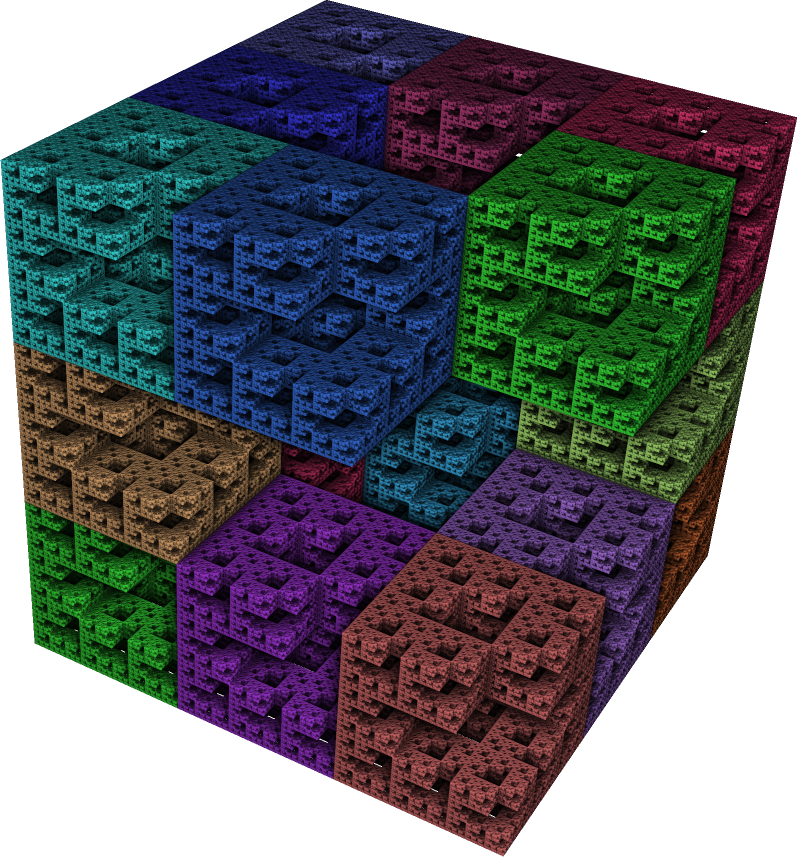
\includegraphics[width=0.45\textwidth]{qK.png}
\hfill
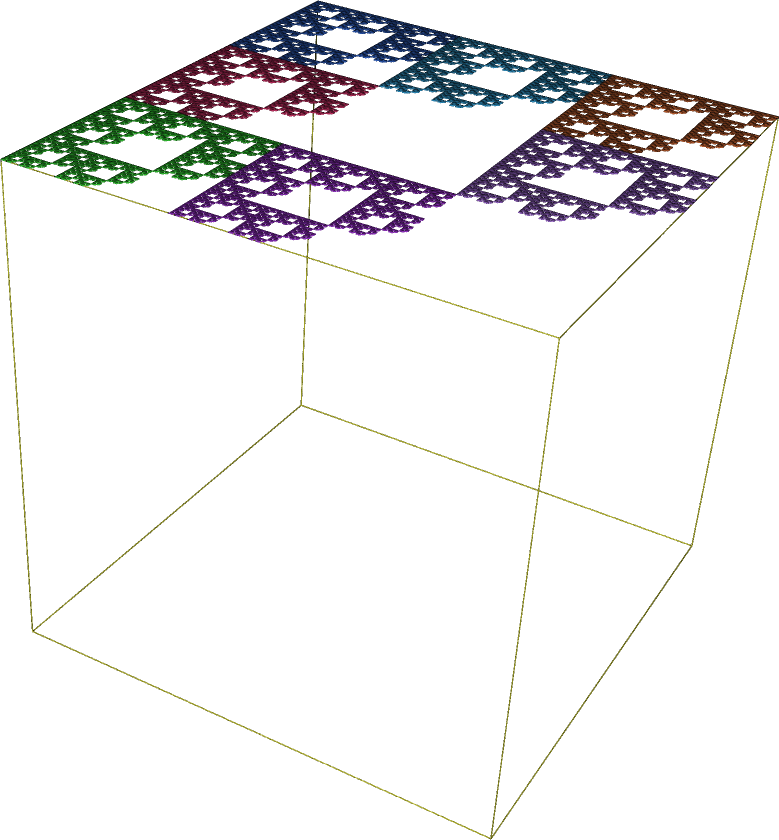
\includegraphics[width=0.45\textwidth]{qK_a.png}}
\only<2>{
\begin{lemma}
Каждая грань $K_\bma$ фрактального куба $K$ сама является фрактальным кубом, удовлетворяющим уравнению $K_\bma=\dfrac{K_\bma+D_\bma}{n}$ с множеством единиц $D_\bma:=D\cap(n-1)P_\bma$.
\end{lemma}
\centering{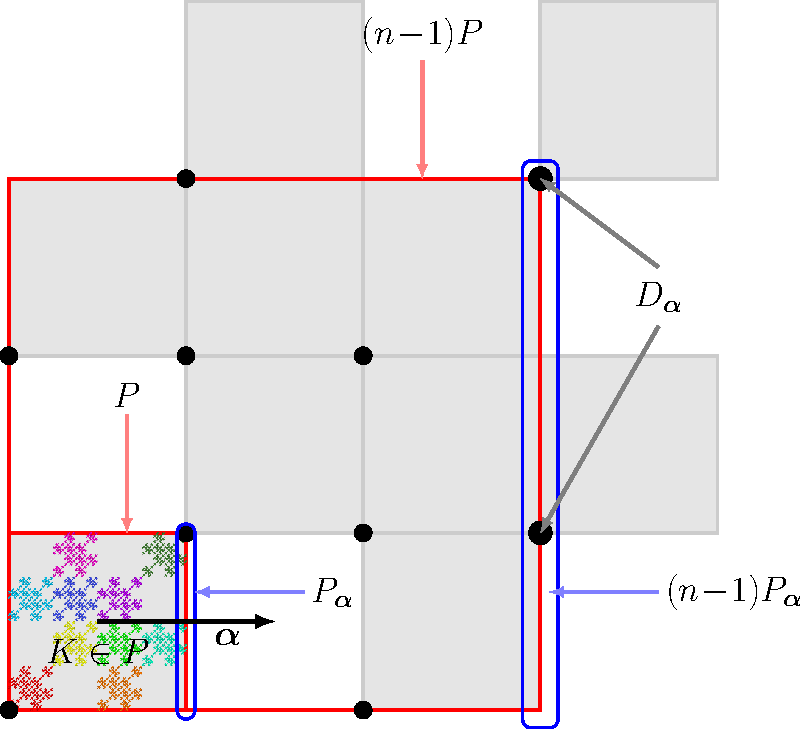
\includegraphics[width=0.5\textwidth]{ffaces.pdf}}
}
\end{frame}


\begin{frame}{Теорема о пересечениях фрактальных $k$-кубов}
\begin{definition}
Пусть $K^1,K^2$ --- фрактальные $k$-кубы порядка $n$ с множествами единиц $D^1,D^2$.
Обозначим их пересечения как $F_0:=K^1\cap K^2$ и $F_\bma:=K^1\cap (K^2+\bma)$, где $\bma\in A$.
\end{definition}
Поскольку   $K_{\bma}^1=K^1\cap  P_\bma$ и $K_{-\bma}^2=K^2\cap P_{-\bma}$ , то $F_\bma=K_{\bma}^1\cap(K_{-\bma}^2+\bma)$.
% *ДОБАВИТЬ ПО НОРМАЛЬНОМУ $Q_\alpha=\dfrac{Q_\alpha+D_\alpha}{n}$
\begin{theorem}
Семейство $\{F_\bma, \bma\in A\}$ пересечений $F_\bma =K_{1}\cap (K_{2}+\bma)$  
удовлетворяет системе уравнений
\begin{equation*}
\left\{F_\bma=\bigcup\limits_{\bmb\sqsupseteq{\bma}}T_{\bma\bmb}(F_\bmb),\qquad \bma\in A,\right\}
\end{equation*}
где для любого $\bmb\sqsupseteq\bma$ $T_{\bma\bmb}(F_\bmb)=\frac{1}{n}(F_\bmb+G_{\bma\bmb})$ и $G_{\bma\bmb}=D_1\cap(D_2+n\bma-\bmb)$.\\
\end{theorem}
\end{frame}


\begin{frame}{Структурный граф}
% *Вершина $\beta$ подчинена $\alpha$
% ?конечное/счетное/несчетное пересечение
% ?Несвязный граф = не используемая стыковка
\centering{
    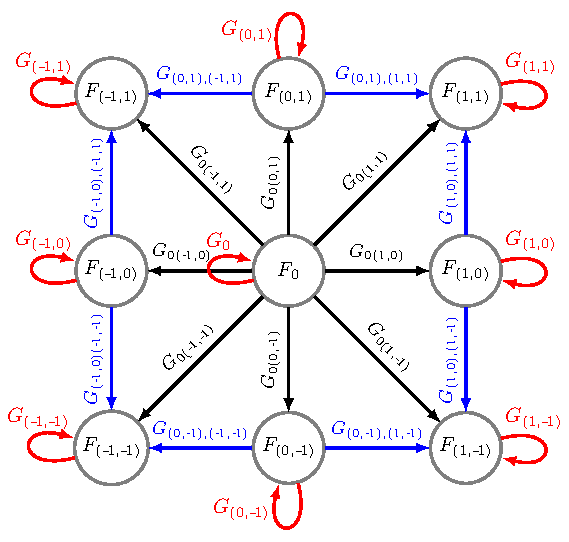
\includegraphics[width=0.65\textwidth]{structure_grapg_full.pdf}}
\end{frame}

\begin{frame}{Мощность пересечения $F_\bma$}
\begin{definition}
Мы говорим, что пара вершин $F_\bma, F_\bmb, \bma\sqsubset\bmb$ {\em соединена направленным путем} в графе $\Ga_\Sa$, если существует конечная последовательность  $\bma=\bma_0\sqsubset\bma_1\sqsubset\ldots \bma_{p-1}\sqsubset\bma_p=\bmb$ такая, что для любых  $j=0,\ldots  ,p$ множества $F_{\bma_j}\neq\0$  и множества $G_{\bma_{j-1}\bma_j}\neq\0$ для $j=1,\ldots  ,p$.   
\end{definition}

Мы пишем $\bmb\succ\bma$, если в $\Ga$ есть направленный путь от $F_\bma$ до $F_\bmb$.
\begin{theorem}
\begin{enumerate}%[nolistsep]
\item[1] Множество $F_\bma$ является одноточечным, если $\Gamma_\bma$ представляет собой цепочку $\bma=\bma_1\prec\ldots\prec\bma_p$, в которой для всех $j\le p-1$, $\# G_{\bma_j\bma_{j+1}}=1$, $G_{\bma_j}=\0$ и $\#G_{\bma_p}=1$;
\item[2] Множество $F_\bma$ конечно, если для всех максимальных вершин $\bmb$ в $\Gamma_\bma$, верно $\#G_\bmb=1$ и $G_{\bmb}=\0$ для всех остальных вершин в $\Gamma_\bma$.
В этом случае $\#F_\bma$ равно сумме всех композиций $\prod \limits_{j=1}^{p-1}\# G_{\bma_j\bma_{j+1}}$, взятых по всем цепочкам $\bma=\bma_1\prec\ldots\prec\bma_p=\bmb$, где $\bmb$ является максимальным в $\Gamma_\bma$;
\item[3] Множество $F_\bma$ счетно, если $\#G_\bmb\le 1$ для всех вершин $\bmb$ в $\Gamma_\bma$;
\item[4] Множество $F_\bma$ несчетно, если в $\Gamma_\bma$ существует такая вершина $\bmb$, что $\#G_\bmb> 1$.
\end{enumerate}
\end{theorem}
\end{frame}


\begin{frame}{Пересечение фрактальных квадратов по 78 точкам}
\only<1>{
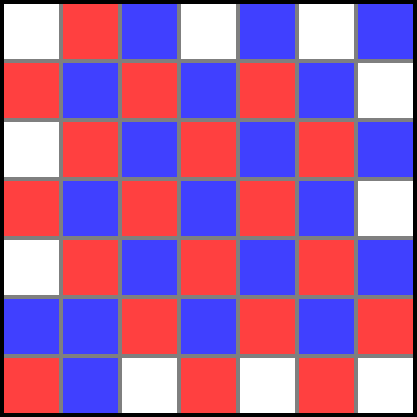
\includegraphics[width=0.45\textwidth]{FSI_7x7_DS.pdf}
\hfill
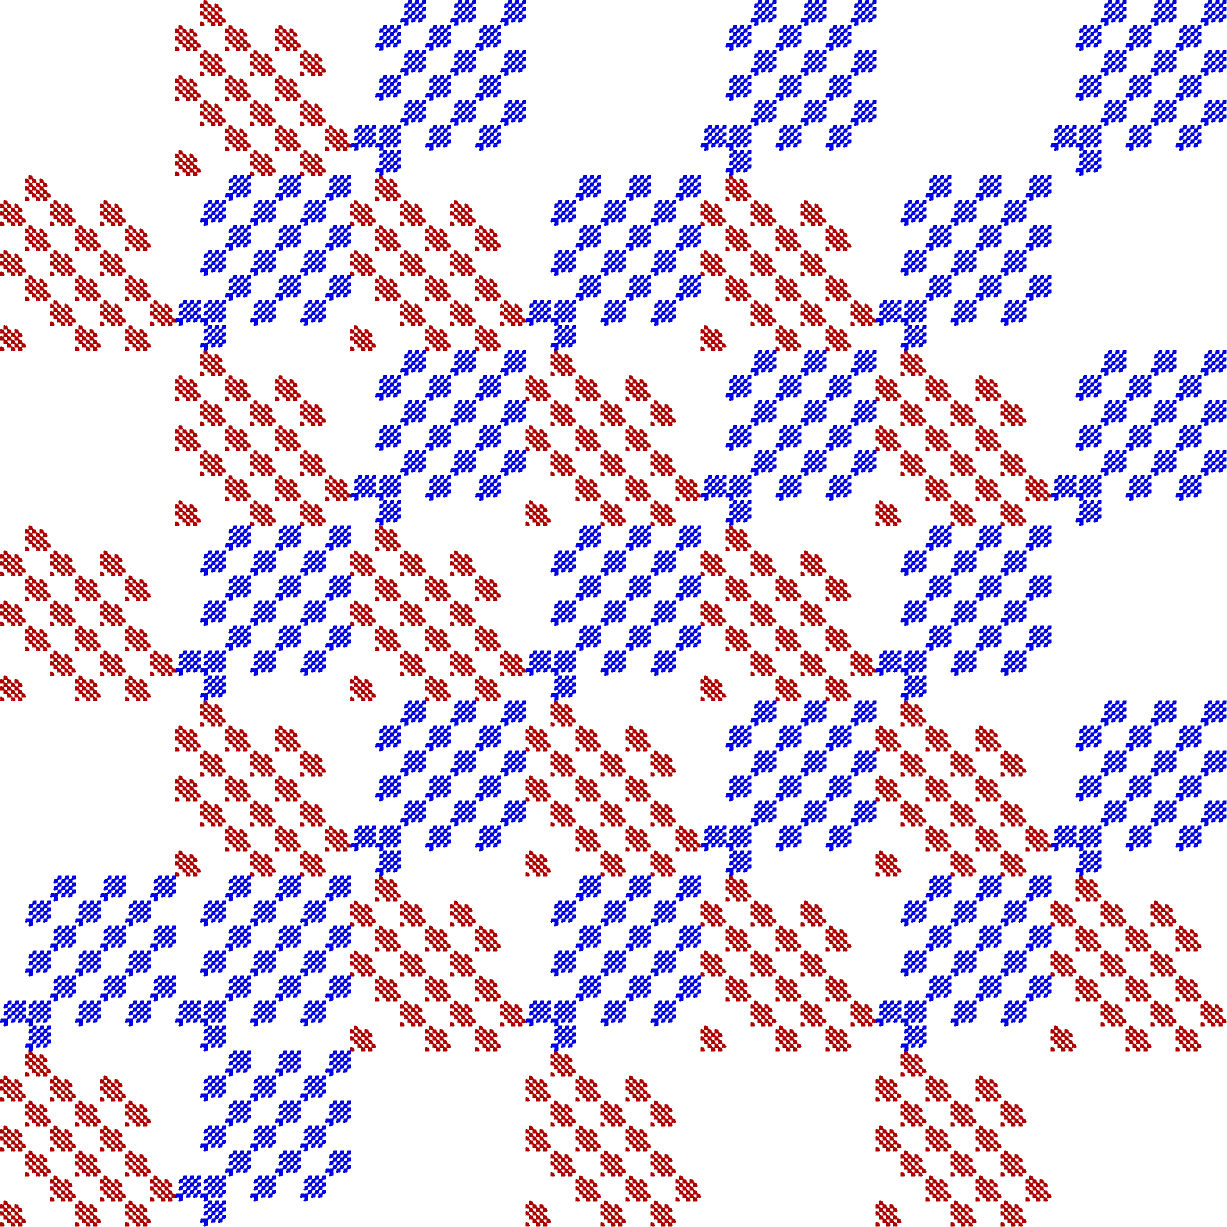
\includegraphics[width=0.45\textwidth]{FSI_7x7_K.png}}
\only<2>{
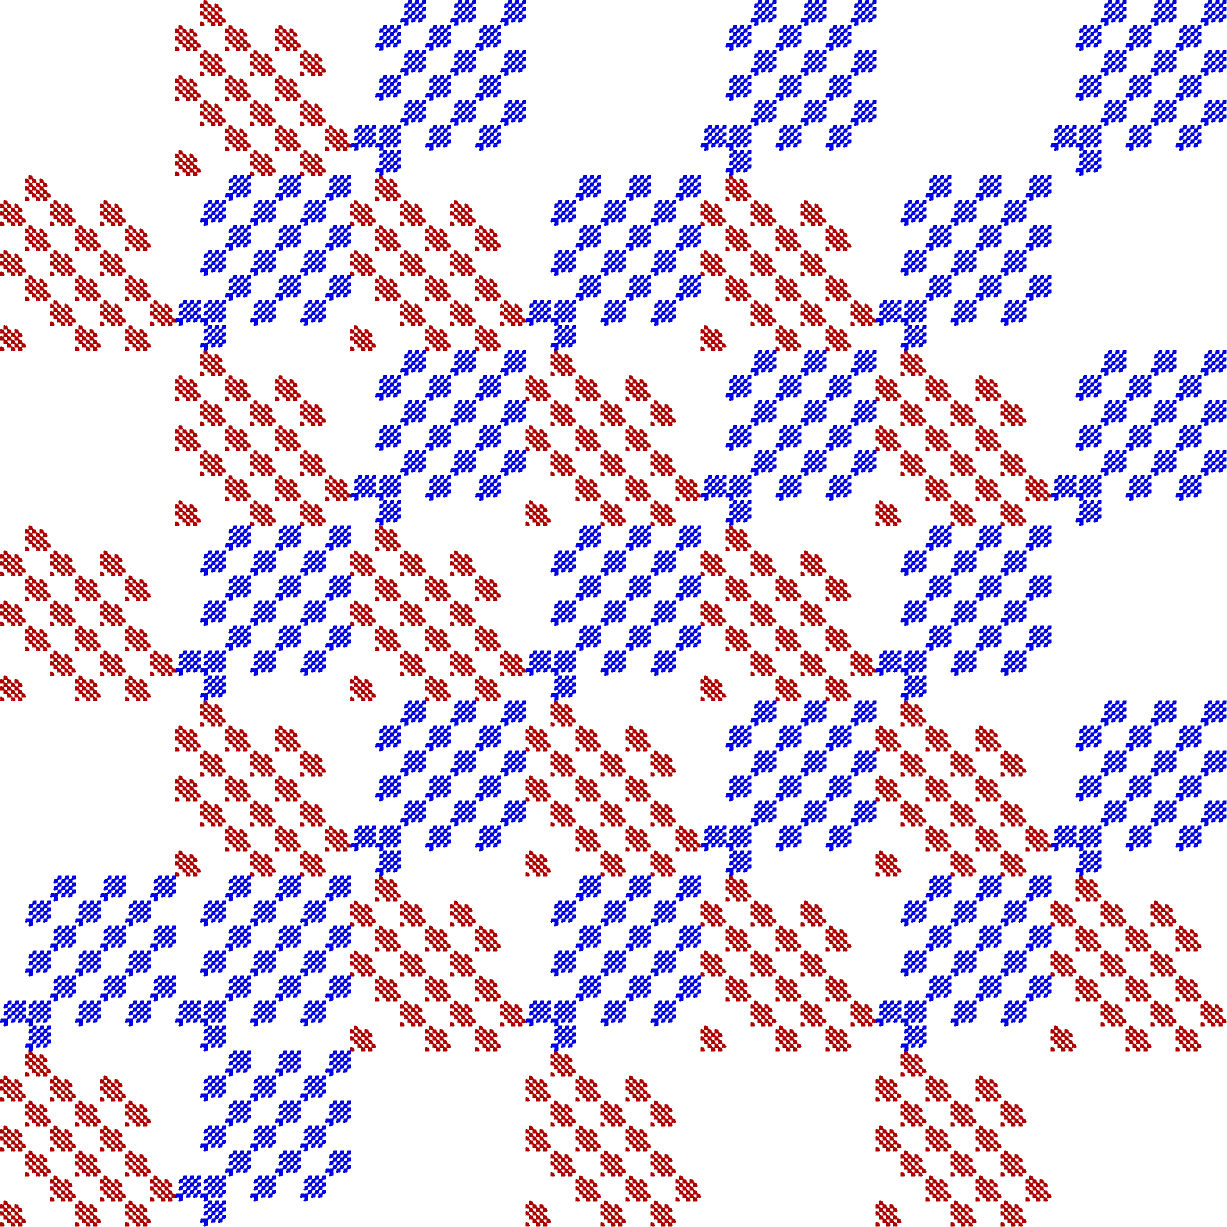
\includegraphics[width=0.45\textwidth]{FSI_7x7_K.png}
\hfill
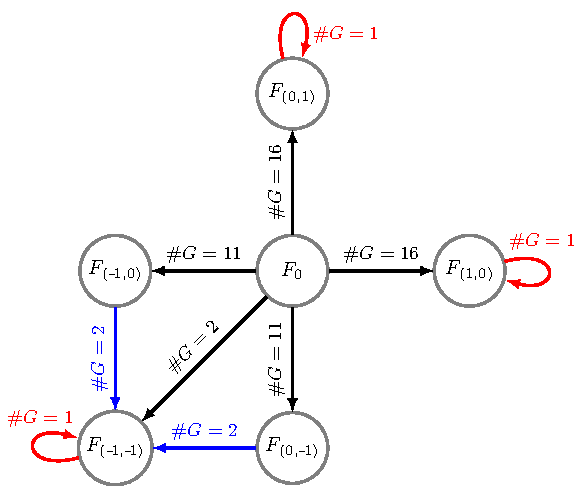
\includegraphics[width=0.45\textwidth]{FSI_7x7_SG.pdf}}
\end{frame}

\begin{frame}{Теорема о бесконечной мере}
\begin{remark}
Обозначим  фрактальный куб с множеством единиц $G_{\bma\bma}$ как $Q_\bma$.
Он удовлетворяет выражению $Q_\bma=\frac{1}{n}(Q_\bma+G_{\bma\bma})$, а значит $\dim_H(Q_\bma)=\log_n\#G_{\bma\bma}$.
\end{remark} 

\begin{definition}
Для каждого $\bma\in A$ обозначим  $\nu(\bma)=\max\{\#G_{\bmb\bmb} : \bmb\succcurlyeq\bma\}$ и $s(\bma)=\log_n\nu(\bma)$.   
\end{definition}

\begin{lemma}
Если $\#G_0=\#G_\bma=l$, $\log_nl=s$ и для любого $\bmb\succ 0$ верно $\#G_\bmb\le l$, то $H^s(F_0)$ бесконечна.
\end{lemma}
\end{frame}

\begin{frame}{Пересечение фрактальных квадратов с $\dim_H(F_0)=1$ и $H^1(F_0)=\infty$}
\only<1>{
\begin{columns}
    \column{0.3\textwidth}
    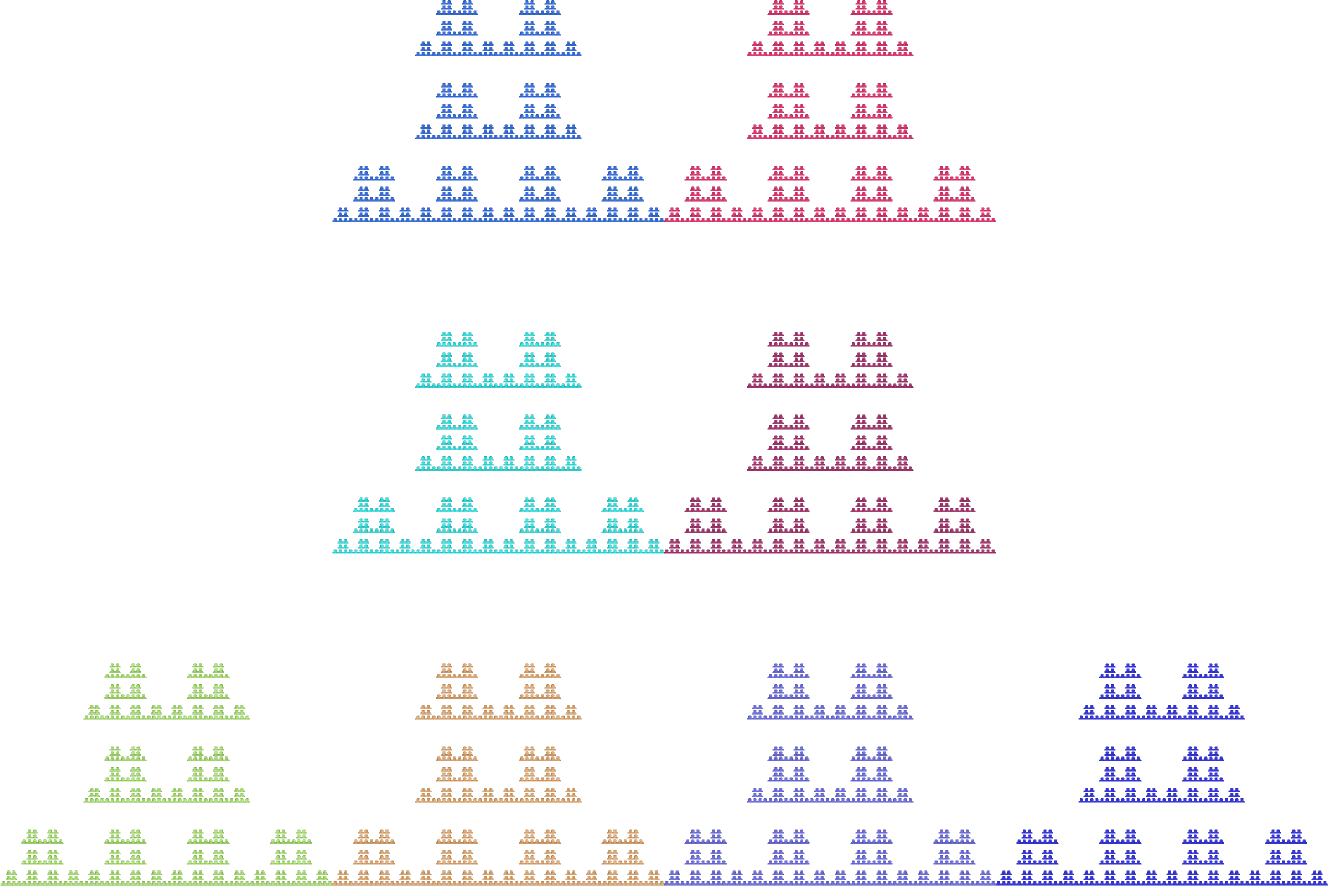
\includegraphics[width=\textwidth]{e1K1.png}\\ \vspace{0.5cm}
    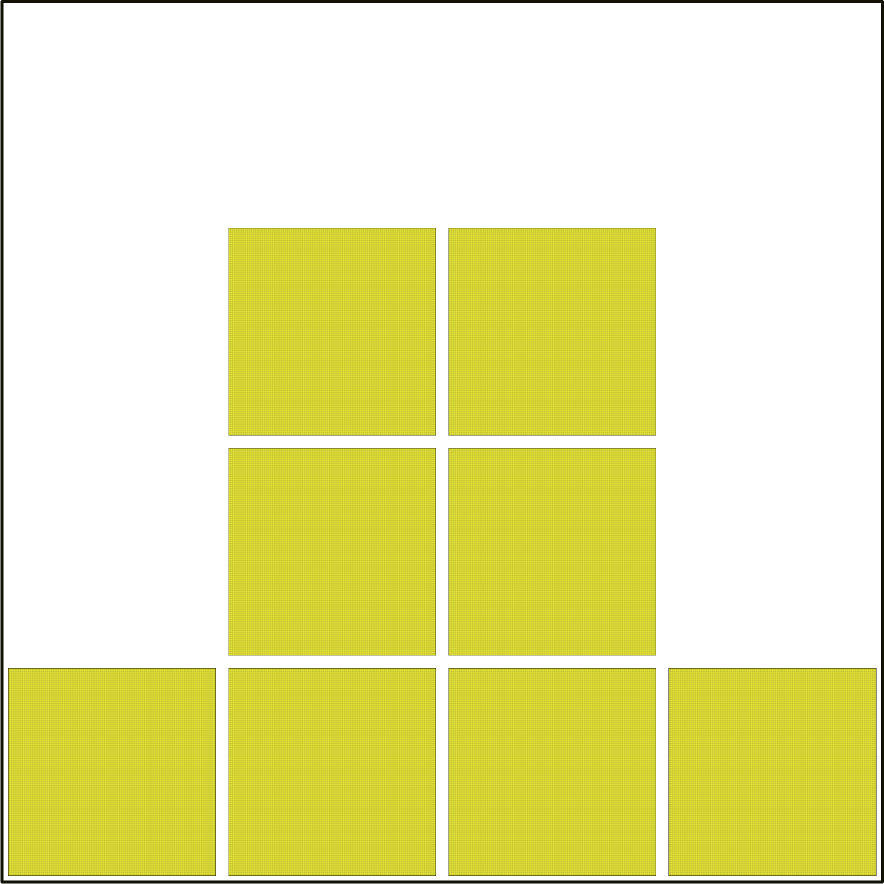
\includegraphics[width=\textwidth]{e1P1.png}
    \column{0.3\textwidth}
    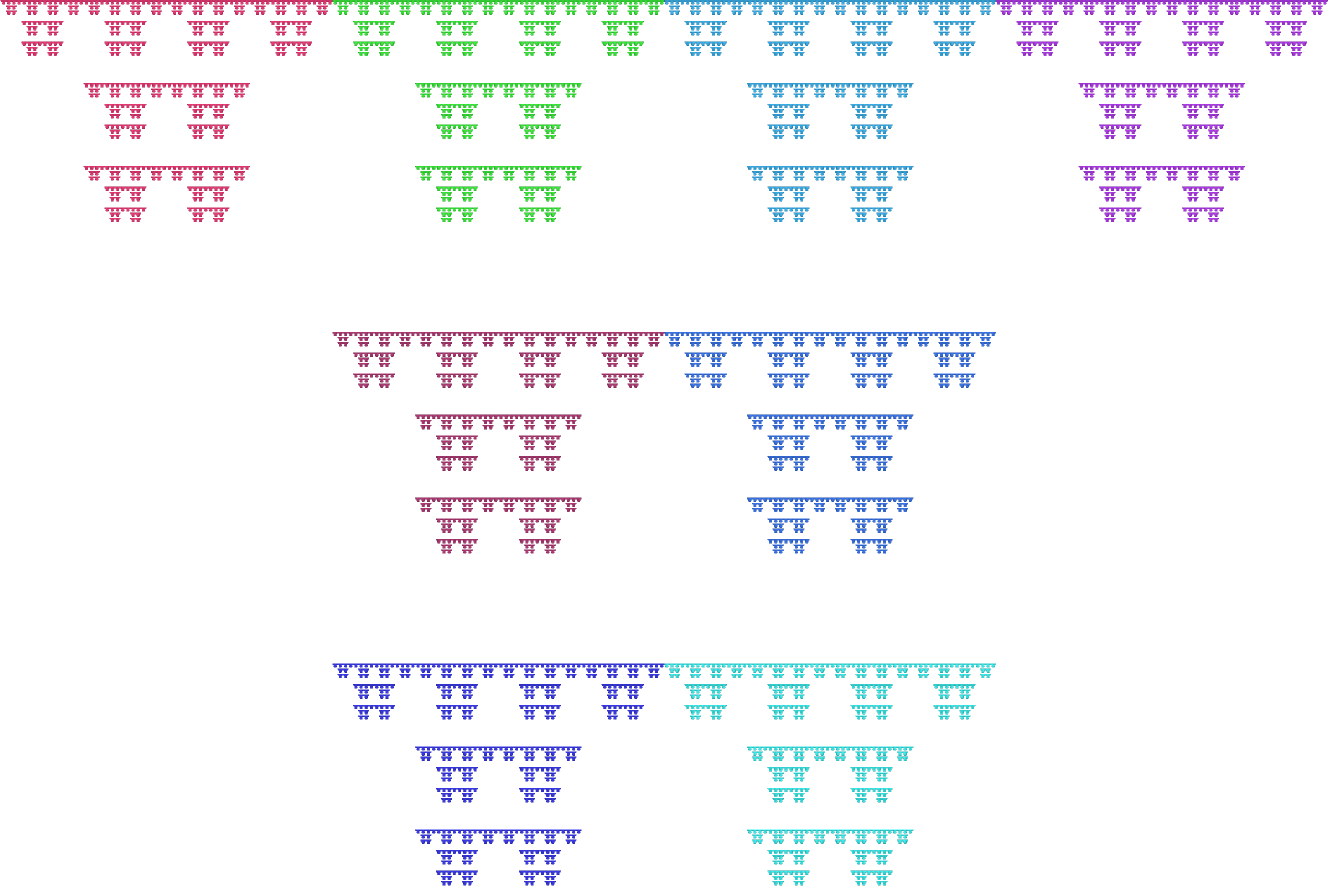
\includegraphics[width=\textwidth]{e1K2.png}\\ \vspace{0.5cm}
    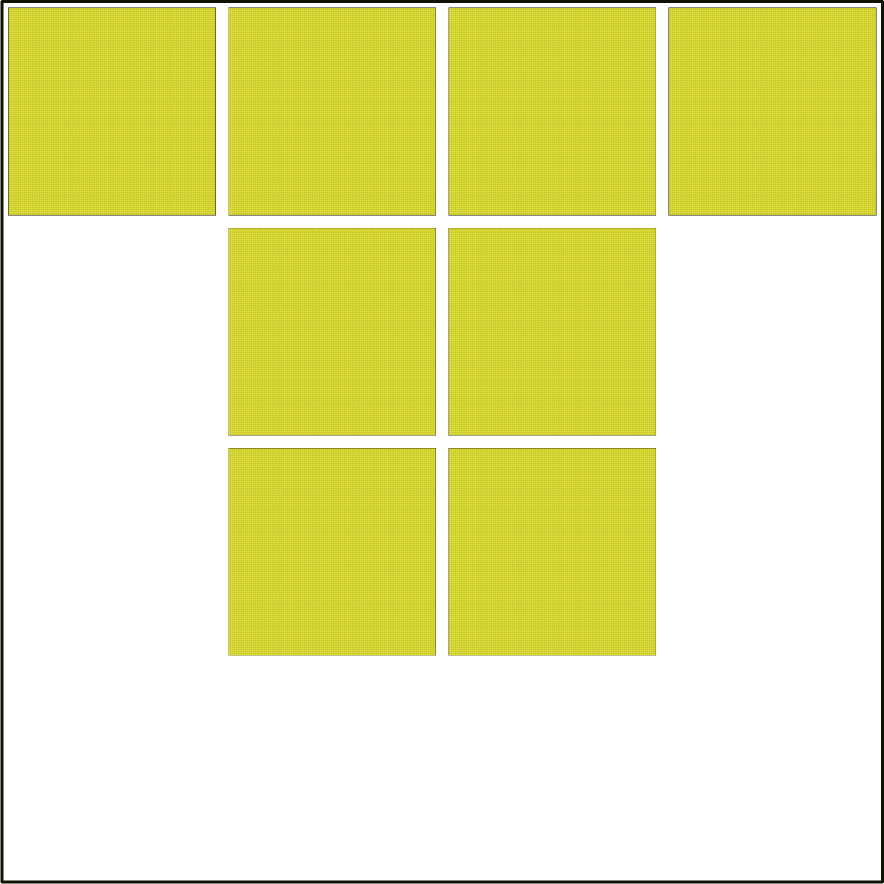
\includegraphics[width=\textwidth]{e1P2.png}
\end{columns}\vspace{.5 cm}
\centering{Фрактальные квадраты $K_1,K_2$ при $\#G_0=4$ и $\#G_{(0,-1)}=4$.}
}
\only<2>{
\begin{columns}
\column{0.5\textwidth}
    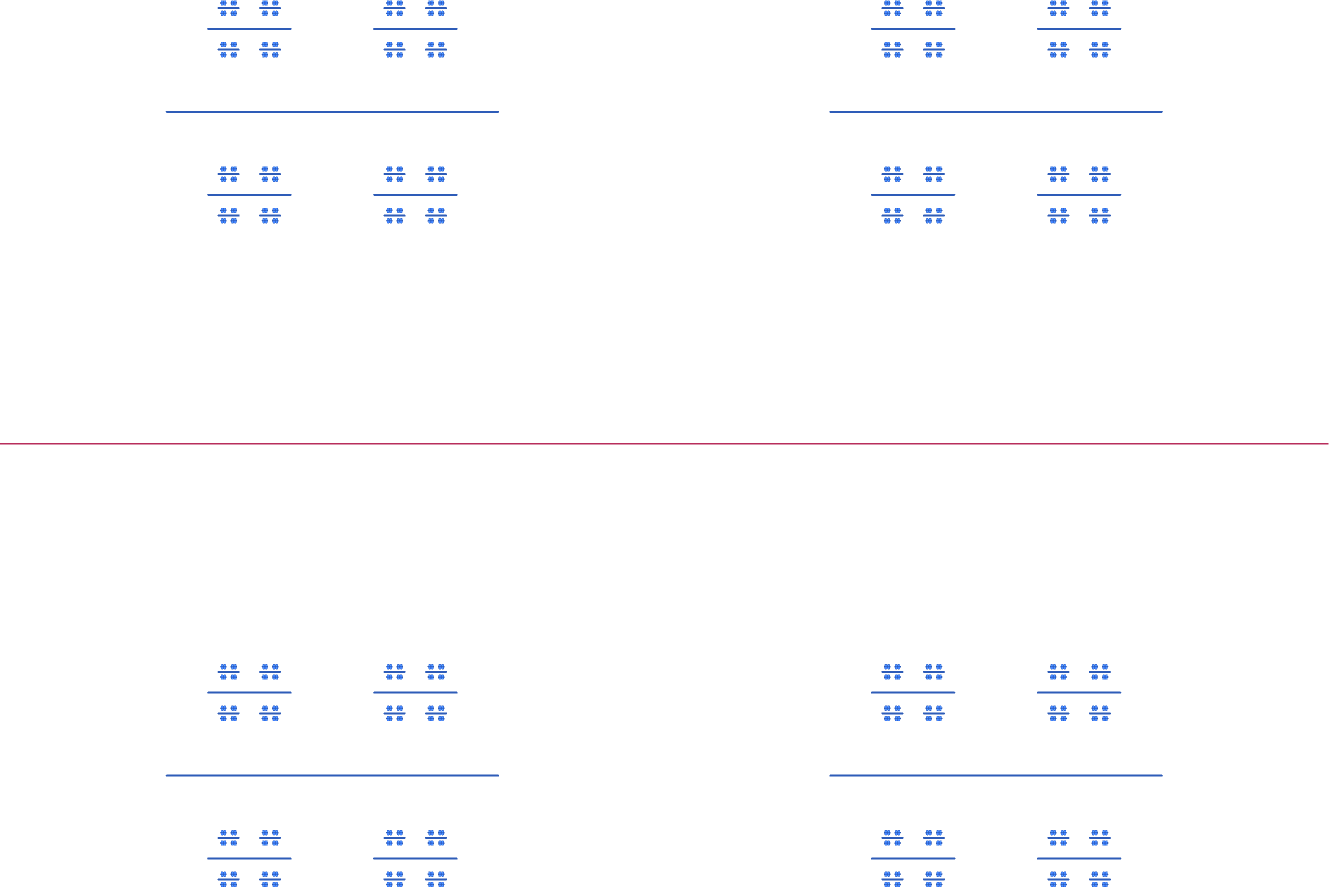
\includegraphics[width=\textwidth]{e1K12.png}
    \column{0.5\textwidth}
    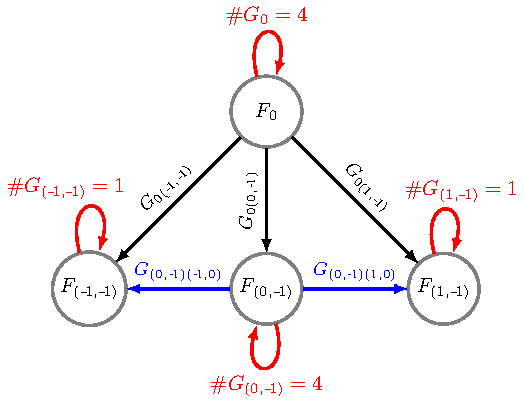
\includegraphics[width=\textwidth]{sg_GDS_InfM.pdf}
\end{columns} \vspace{0.5cm}
\begin{columns}
    \column{0.5\textwidth}
    \centering{Пересечение $F_0=K_1\cap K_2$}
    \column{0.5\textwidth}
    \centering{Структурный граф $\Ga$ для $K_1\cap K_2$}
\end{columns}}
\end{frame}


\begin{frame}{}
\Huge{Часть 3.\\
Классификация фрактальных квадратов, являющихся дендритами}
\end{frame}

\begin{frame}{Цели и выносимые на защиту положения}
Цель:
\begin{enumerate}
\item[$\bullet$] Проверить, при каких условиях фрактальный квадрат является дендритом. Можно ли получить дендрит с неодноточечным пересечением.
\item[$\bullet$] Перечислить все формы главных деревьев фрактальных квадратов, являющихся дендритами.
\end{enumerate}

\hfill

Выносимые на защиту положения:
\begin{enumerate}
\item[1] Фрактальный квадрат $K$ является дендритом тогда и только тогда, когда его двудольный граф пересечений является деревом, а значит такие дендриты могут быть только с одноточечным пересечением;
\item[2] Для фрактальных квадратов, являющихся дендритами, существует только $7$ типов главного дерева.
\end{enumerate}
\end{frame}

\begin{frame}{Самоподобная граница}
\only<1>{
    \begin{definition}
    {\em Критическое множество} аттрактора $K$ системы $\eS$ --- это множество $C:=\{x:\; x\in S_i(K)\cap S_j(K),\; S_i, S_j\in\eS\}$ точек попарных пересечений копий аттрактора $K$.
    \end{definition}
    \begin{definition}
    {\em Самоподобной границей} аттрактора $K$ называется множество $\dd K$ всех $x\in K$ таких, что для некоторого $\bj\in I^*$ верно $S_\bj(x)\in C$.
    \end{definition}}
%\only<2>{Вставить картинку с треугольником Серпинского, его критическим множеством и самоподобной границей}
\end{frame}

\begin{frame}{Простой граф пересечений}
\begin{definition}
Обозначим как $\tilde{\Gamma}(\eS)$ граф, вершинам которого соответствуют копии $\{K_i:\; i\in I\}$, а пара вершин $K_i,K_j$ соединена ребром, если $K_i\cap K_j\neq\0$.
Назовём такой граф {\em простым графом пересечений} для $K(\eS)$ 
\end{definition}

\begin{theorem}[Критерий связности, Hata M. (1985)]
Аттрактор $K$ системы $\eS$ связен тогда и только тогда, когда его простой граф пересечений $\tilde{\Gamma}(\eS)$ связен.
\end{theorem}
\footnotetext[5]{Hata Masayoshi, On the structure of self-similar sets, Japan Journal of Applied Mathematics 2 (1985), 381--414.}
% \footnotetext[2]{Bandt C. and Keller K., Self-Similar Sets 2. A Simple Approach to the Topological Structure of Fractals, Mathematische Nachrichten 154, 1(1991), 27--39}
\end{frame}


\begin{frame}{Двудольный граф пересечений}
\only<1>{
\begin{definition}
Пусть множество $K=K(\eS)$ --- самоподобный континуум, обладающий свойством одноточечного пересечения.
{\em Граф пересечений} $\Gamma(\eS)$ системы $\eS$ --- это двудольный граф с долями $\eK=\{K_i:\; i\in I\}$ и $\eP=\{p:\;p\in K_i\cap K_j,\; i,j\in I, i\neq j\}$, и с множеством рёбер $E=\{(K_i,p):p\in K_i\}$.
\end{definition}
Мы называем $K_i\in \eK$ {\em белыми вершинами}, а $p\in \eP$   {\em чёрными вершинами} графа $\Ga$.\\

Набор компактов $\mathcal{A}=\{A_i,i\in I\}$ в $\mathbb{R}^n$ называют {\em системой со свойством одноточечного пересечения}, если для любых $i\neq j\in I$, пересечение $P_{ij}=A_i\cap A_j$ не более чем одноточечно.


%\begin{definition}
%{\em Дендрит} --- это локально связный континуум, не содержащий простых замкнутых дуг
%\end{definition}
\begin{theorem}[Tetenov A. V. (2021)]
Пусть $K=K(\eS)$ --- самоподбный континуум со свойством одноточечного пересечения.
Если граф пересечений $\hat\Gamma(\eS)$ системы $\eS$ является деревом, то её аттрактор $K$ --- дендрит.
\end{theorem}
\footnotetext[6]{Tetenov A., Finiteness properties for self-similar continua, arXiv:2003.04202 (2021)}}
\only<2>{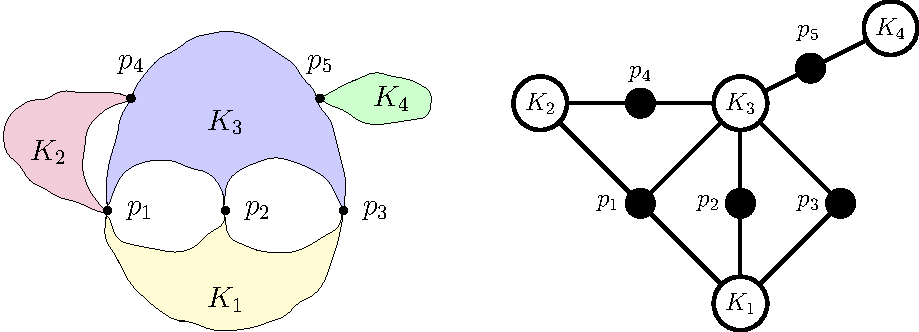
\includegraphics[width=\textwidth]{IG_for_FIP.pdf}}
\end{frame}

\begin{frame}{Двудольный граф пересечений для фрактального квадрата дендрита}
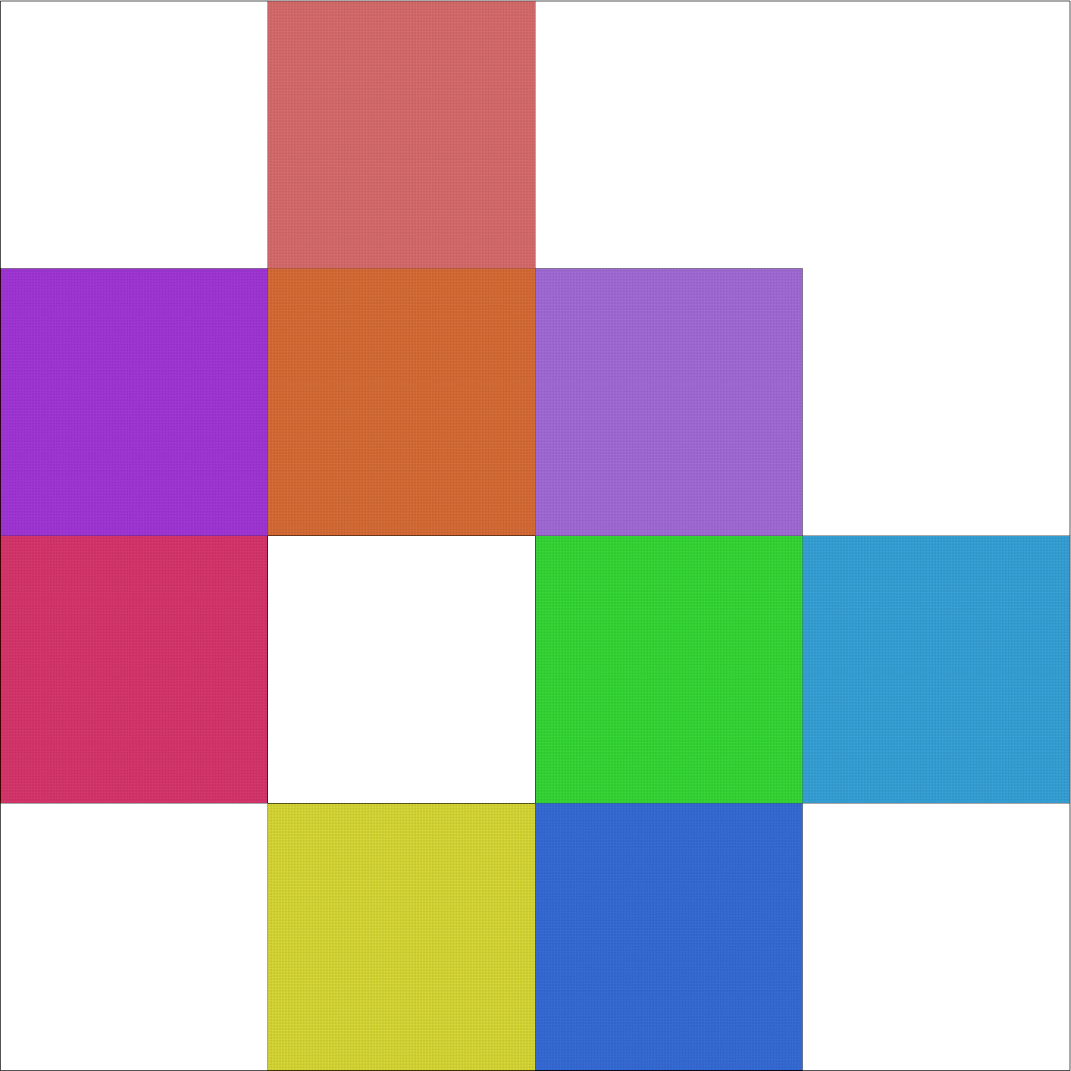
\includegraphics[width=0.3\textwidth]{P1.png}
\hfill
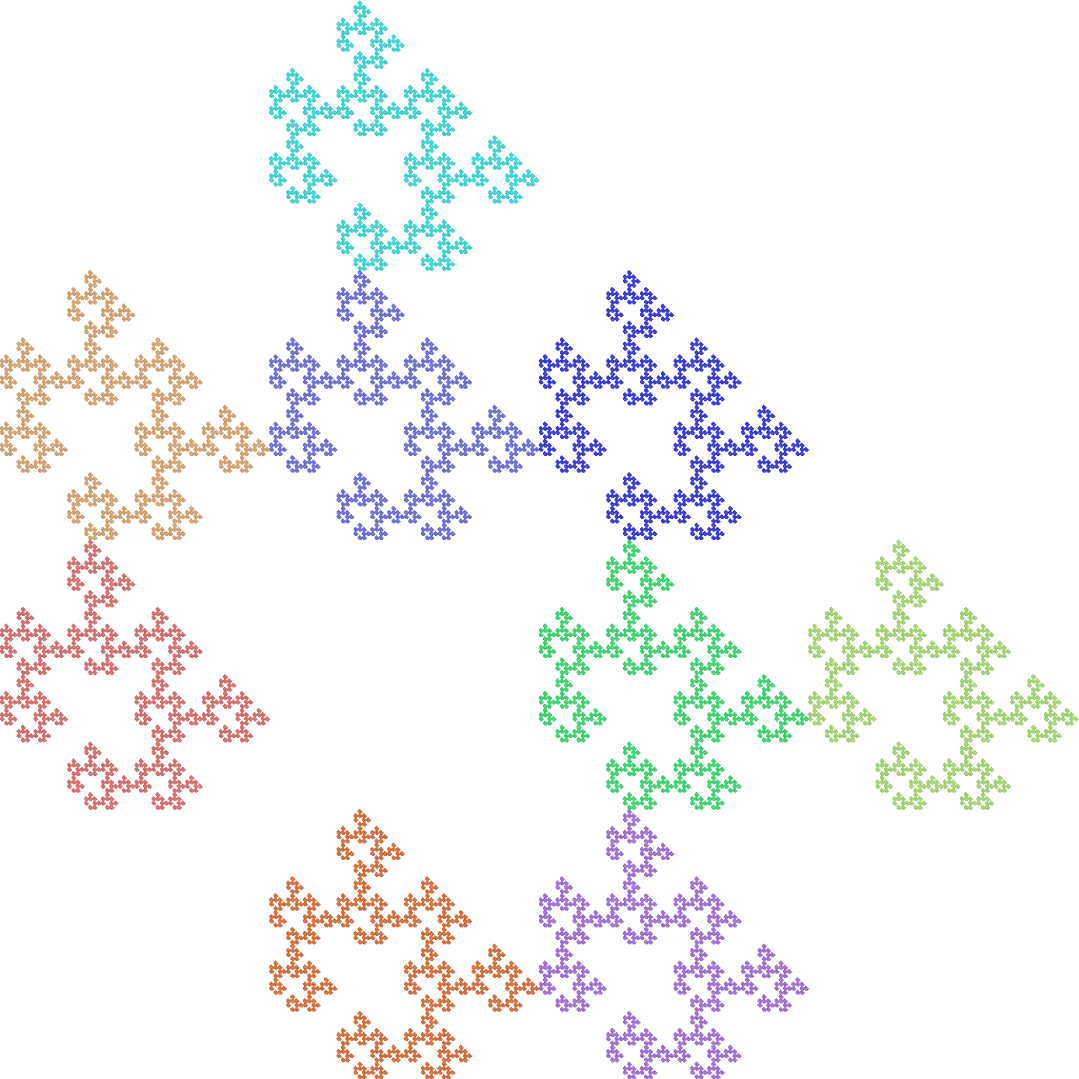
\includegraphics[width=0.3\textwidth]{presentation/K.png}
\hfill
\includegraphics[width=0.3\textwidth]{FS_PIG.pdf}

\end{frame}




\begin{frame}{Критерий дендритности фрактального $k$-куба}
\begin{theorem}
Фрактальный квадрат $K$ является дендритом тогда и только тогда, когда его двудольный граф пересечений является деревом.
\end{theorem}
\vspace{0.5cm}
\center{
\includegraphics[width=0.8\textwidth]{line_int.png}}
\end{frame}


\begin{frame}{Классификация фактальных квадратов дендритов}
\begin{definition}
Пусть $K$ --- самоподобный дендрит, обладающий конечной самоподобной границей $\dd K$. 
Минимальный поддендрит $\hat\gamma\IN K$, содержащий $\dd K$, называется {\em главным деревом} дендрита $K$.
\end{definition}
\begin{theorem}\label{thm:tree_classes}
% The fractal square dendrites may be divided to $7$ types depending on the form of their main tree.
Для фрактальных квадратов, являющихся дендритами, существует только $7$ типов главного дерева, модели которых показаны ниже.
\end{theorem}
\includegraphics{mt1.pdf}
\hfill
\includegraphics{mt2.pdf}
\hfill
\includegraphics{mt3.pdf}
\hfill
\includegraphics[width=2.2cm]{mt4.pdf}\\
\includegraphics[width=2.5cm]{mt5.pdf}
\hfill
\includegraphics[width=2.3cm]{mt6.pdf}
\hfill
\includegraphics[width=3.2cm]{mt7.pdf}
\end{frame}

\begin{frame}{Типы фрактальных квадратов дендритов и их самопообная граница}
\large
\begin{lemma}\label{ssboundary}
% Let $K$ be a fractal square dendrite which is not a line segment.\\ Then its self-similar boundary $\dd K$ belongs to one of the following types:\\

% $\dd K=F_\bma\cup F_{-\bma}\cup F_\bmb\cup F_{-\bmb}$, where\\
% {\bf (A)} $\bma=(1,0),\bmb=(0,1)$;\\
% {\bf (B)} $\bma=(1,1),\bmb=(1,-1)$;\\
% {\bf (C)} $\bma=(1,1) \mbox{ or } (1,-1),\bmb=(1,0) \mbox{ or  }(0,1)$;\\

% or {\bf (D)} $\dd K=F_{(1,0)}\cup F_{(-1,0)}\cup F_{(0,1)}\cup F_{(0,-1)}\cup F_\bmb\cup F_{-\bmb}$ \\where
% $\bmb=(1,1) \mbox{ or  }(1,-1)$. \\

% In the cases {\bf A,B,C} the set $\dd K$ consists of 4 points.\\
% In the case {\bf D} the set $\dd K$ may consist of 3 or 6 points.
Пусть $K$ --- фрактальный квадрат, являющийся дендритом и не являющийся отрезком прямой. 
Тогда его самоподобная граница $\dd K$ описывается следующим образом:\\
$\dd K=F_\bma\cup F_{-\bma}\cup F_\bmb\cup F_{-\bmb}$, где\\
{\bf (A)} $\bma=(1,0), \bmb=(0,1)$;\\
{\bf (B)} $\bma=(1,1), \bmb=(1,-1)$;\\
{\bf (C)} $\bma=(1,1)$ или $(1,-1)$,\qquad\;$\bmb=(1,0)$ или $(0,1)$;\\
или {\bf (D)} $\dd K=F_{(1,0)}\cup F_{(-1,0)}\cup F_{(0,1)}\cup F_{(0,-1)}\cup F_\bmb\cup F_{-\bmb}$ где $\bmb=(1,1)$ или $(1,-1)$. 
В случаях {\bf A, B, C} множество $\dd K$ состоит из $4$ точек.
В случае {\bf D} множество $\dd K$ может состоять из $3$ или $6$ точек.
\end{lemma}
\end{frame}


\begin{frame}{
\only<1>{Тип \textbf{A}}
\only<2>{Тип \textbf{B}}
\only<3>{Тип \textbf{C}}
\only<5>{Тип \textbf{D3}}
\only<4>{Тип \textbf{D6}}}
\begin{center}
\only<1>{\includegraphics[width=0.6\textwidth]{A_type.pdf}}
\only<2>{\includegraphics[width=0.6\textwidth]{B_type.pdf}}
\only<3>{\includegraphics[width=0.6\textwidth]{C_type.pdf}}
\only<5>{\includegraphics[width=0.6\textwidth]{D3_type.pdf}}
\only<4>{\includegraphics[width=0.6\textwidth]{D6_type.pdf}}
\end{center}
\end{frame}


\begin{frame}{Порядок ветвления произвольной точки}
\only<1>{
\begin{theorem}
Для любой точки $x$ во фрактальном квадрате $K=\dfrac{D+K}{n}$, являющимся дендритом, верно, что $Ord(x,K)\le 4$.
\end{theorem}
\includegraphics[width=\textwidth]{case1.pdf}}
\only<2>{\includegraphics[width=\textwidth]{case2.pdf}}
\only<3>{\center{\includegraphics[width=0.8\textwidth]{case3.pdf}}}
\end{frame}


\begin{frame}{Порядок ветвления угловой точки
\only<2>{ в \textbf{A}}\only<3>{ в \textbf{C}}\only<4>{ в \textbf{D6}}}
\only<1>{
\begin{theorem}
Пусть $K$ --- фрактальный квадрат, являющийся дендритом.
Если $a\in K$ есть угловая точка, то $Ord(a,K)\leq 2$.
\end{theorem}

\begin{theorem}
Пусть $K$ --- фрактальый квадрат, являющийся дендритом. \\
В случае {\bf A} у $K$ может быть две угловые точки с порядками ветвления $\le 2$, или $1$ угловая точка с порядком  $\le 2$, или вовсе не быть угловых точек.\\
В случае {\bf B} у $K$ всегда четыре угловых точки с порядками ветвления $1$.\\
В случае {\bf C} у $K$ всегда две угловых точки с порядками ветвления $\le 2$\\
В случае {\bf D} у $K$ может быть либо две угловых точки с порядками ветвления $\le 2$, либо три угловых точки с порядками ветвления $1$.
\end{theorem}}
\only<2>{\includegraphics[width=\textwidth]{A_type_Three.png}}
\only<3>{\includegraphics[width=\textwidth]{C_type_Three.png}}
\only<4>{\includegraphics[width=\textwidth]{D6_type_Three.png}}
\end{frame}




\begin{frame}{Порядок точки ветвлния в главном дереве в \textbf{(D6)}}
\only<1>{
\begin{proposition}\label{lem:d4bound}
Пусть $K$ --- фрактальный квалрат типа  {\bf D6}  и $\gamma$ --- его главное дерево.\\ 
 (i)  для любого $x\in\dd K$ верно, что $Ord(x,\gamma)\leq2$;\\
(ii) для любого $x\in\gamma$ верно, что $Ord(x,K)\leq3$.
\end{proposition}
\vspace{1cm}
\includegraphics[width=\textwidth]{d6ord3full.pdf} }
%\only<2>{\includegraphics[width=\textwidth]{d6ord3_12.pdf} }
%\only<3>{\includegraphics[width=\textwidth]{d6ord3_34.pdf} }
\end{frame}


\begin{frame}{}
\frametitle{
    \only<1>{Дерево 1: классы 1 (\textbf{A}) и 2 (\textbf{C})}
    \only<2>{Дерево 2: классы 3 (\textbf{A}), 4 (\textbf{A}), 5 (\textbf{C}) и 6 (\textbf{D3})}
    \only<3>{Дерево 3: классы 7 (\textbf{A}), 8 (\textbf{B}) и 9 (\textbf{C})}
    \only<4>{Дерево 4: классы 10 (\textbf{A}), 11 (\textbf{B}), 12 (\textbf{C}) и 13 (\textbf{D6})}
    \only<5>{Дерево 5: класс 14 (\textbf{D6})}
    \only<6>{Дерево 6: класс 15 (\textbf{D6})}
    \only<7>{Дерево 7: класс 16 (\textbf{D6})}}
\only<1>{
    \center{\includegraphics[scale=1.5]{mt1.pdf}
    \vspace{0.5cm}
    \vfill
    \fbox{
    \includegraphics[width=0.22\textwidth]{1K.png}
    \includegraphics[width=0.22\textwidth]{1T.png}}
    \hfill
    \fbox{
    \includegraphics[width=0.22\textwidth]{2K.png}
    \includegraphics[width=0.22\textwidth]{2T.png}}}}
\only<2>{
    \center{
    \includegraphics{mt2.pdf}
    \hfill
    \fbox{
    \includegraphics[width=0.18\textwidth]{3K.png}
    \includegraphics[width=0.18\textwidth]{3T.png}}
    \hfill
    \fbox{
    \includegraphics[width=0.18\textwidth]{4K.png}
    \includegraphics[width=0.18\textwidth]{4T.png}}\\
    \vspace{0.4cm}
    \hspace{2.54cm}\fbox{
    \includegraphics[width=0.18\textwidth]{5K.png}
    \includegraphics[width=0.18\textwidth]{5T.png}}
    \hfill
    \fbox{
    \includegraphics[width=0.18\textwidth]{6K.png}
    \includegraphics[width=0.18\textwidth]{6T.png}}\\
    }}
\only<3>{\center{
    \hspace{0.12\textwidth}
    \includegraphics[scale=1.5]{mt3.pdf}
    \hfill
    \fbox{
    \includegraphics[width=0.22\textwidth]{7K.png}
    \includegraphics[width=0.22\textwidth]{7T.png}}\\
    \vspace{0.6cm}
    \fbox{
    \includegraphics[width=0.22\textwidth]{8K.png}
    \includegraphics[width=0.22\textwidth]{8T.png}}
    \hfill
    \fbox{
    \includegraphics[width=0.22\textwidth]{9K.png}
    \includegraphics[width=0.22\textwidth]{9T.png}}\\
    }}
\only<4>{\center{
    \includegraphics{mt4.pdf}
    \hfill
    \fbox{
    \includegraphics[width=0.17\textwidth]{10K.png}
    \includegraphics[width=0.17\textwidth]{10T.png}}
    \hfill
    \fbox{
    \includegraphics[width=0.17\textwidth]{11K.png}
    \includegraphics[width=0.17\textwidth]{11T.png}}\\
    \vspace{0.5cm}\hspace{2.85cm}
    \fbox{
    \includegraphics[width=0.17\textwidth]{12K.png}
    \includegraphics[width=0.17\textwidth]{12T.png}}
    \hfill
    \fbox{
    \includegraphics[width=0.17\textwidth]{13K.png}
    \includegraphics[width=0.17\textwidth]{13T.png}}\\
    }}
\only<5>{\center{
    \includegraphics[scale=1.4]{mt5.pdf}
    \hfill
    \fbox{
    \includegraphics[width=0.22\textwidth]{14K.png}
    \includegraphics[width=0.22\textwidth]{14T.png}}
    }}
\only<6>{\center{
    \includegraphics[scale=1.4]{mt7.pdf}
    \hfill
    \fbox{
    \includegraphics[width=0.22\textwidth]{15K.png}
    \includegraphics[width=0.22\textwidth]{15T.png}}
    }}
\only<7>{\center{
    \includegraphics[scale=1.2]{mt6.pdf}
    \hfill
    \fbox{
    \includegraphics[width=0.22\textwidth]{16K.png}
    \includegraphics[width=0.22\textwidth]{16T.png}}
    }}
\end{frame}


\begin{frame}{Апробация результатов}
\begin{thebibliography}{9}
\bibitem{adam}
	{\sc Drozdov D., Samuel M., Tetenov A.,}
	{\em On deformation of polygonal dendrites preserving the intersection graph,}
	{The Art of Discrete and Applied Mathematics (2) \textbf{4} (2021) 1--21}
	
\bibitem{dd2018}
	{\sc Drozdov D., Samuel M., Tetenov A.,}
	{\em On $\delta$-deformations of Polygonal Dendrites}
	{Topological Dynamics and Topological Data Analysis. IWCTA 2018. Springer Proceedings in Mathematics \& Statistics 350 (2022)  147--164}
	
\bibitem{aseev}
	{\sc Tetenov A., Drozdov D.,}
	{\em On fractal squares possessing finite intersection property,}
	{Bulletin of National University of Uzbekistan: Mathematics and Natural Sciences (3)\textbf{5} (2022) 164--181}
	
\bibitem{FSC}
	{\sc Drozdov D., Tetenov A., }
	{\em On the classification of fractal square dendrites,}
	{Advances in the Theory of Nonlinear Analysis and Its Application (3) \textbf{7} (2023) 19--96}
	
\bibitem{FQint}
	{\sc Tetenov A., Drozdov D.}
	{\em On the intersection of fractal cubes,}
	{(to appear)}
\end{thebibliography}
\end{frame}


\begin{frame}{}
\begin{center}
\Huge Благодарю за внимание
\end{center}
\end{frame}


\end{document}